\documentclass[12pt]{article}
\usepackage[hmargin=0.7in,vmargin=1.0in]{geometry}
\usepackage{graphicx}
\usepackage{amssymb}
\usepackage{amsmath}
\usepackage{pdflscape}
\usepackage{graphicx}
\usepackage[hyphens]{url}
\usepackage{epstopdf}
\usepackage[table]{xcolor}
\usepackage{hyperref}
\usepackage{caption}
\usepackage{array}
\usepackage{booktabs}
\usepackage{pifont}
\usepackage{tabularx}
\usepackage{appendix}
\usepackage{float}
\usepackage{tikz}
\usepackage{adjustbox}
\usepackage{setspace}
\usepackage{arydshln}
\usepackage{subcaption}
\usepackage{moreverb}
\usepackage{multirow}
\usepackage{fancyhdr}
\usepackage{color, colortbl}
\usepackage{filecontents}
\usepackage{endnotes}
\usepackage{makecell}
\usepackage[authoryear,round]{natbib}
\definecolor{lightcyan}{rgb}{0.88,1,1}
\definecolor{cobalt}{rgb}{0.0, 0.28, 0.67}
\definecolor{lightcobalt}{rgb}{0.6, 0.78, 0.97}
\definecolor{turqouise}{rgb}{0.25, 0.88, 0.82}
\DeclareMathOperator{\rank}{rank}
\newcolumntype{P}[1]{>{\centering\arraybackslash}p{#1}}

\makeatletter
\newcommand{\rsum}{\DOTSB\rsum@\slimits@}
\newcommand{\rsum@}{\mathop{\mathpalette\rsum@@\relax}}
\newcommand{\rsum@@}[2]{\reflectbox{$\m@th#1\sum@$}}
\makeatother

\graphicspath{{../figures/}}

\bibliographystyle{plainnat}
\begin{document}


\title{\bf The Uncertain Volatility Backbone:\\ Displaced-Diffusion Mixtures and a Joint ATM--OTM Calibration for the SPX Smile}
\author{Aryan Gupta}
\date{June 2026}

\maketitle


\bigskip
\noindent

\begin{abstract}
  We fit a three-state displaced-diffusion mixture model---the uncertain volatility backbone---to one-month implied volatility on SPX options across four volatility regimes spanning 2015--2025. We propose a \emph{joint ATM--OTM calibration with interpolation} as the core methodology: the nine parameters per regime are estimated simultaneously against empirical IV at three training moneyness levels ($k \in \{-0.20, 0, +0.20\}$), and the smile's intermediate convexity is tested by interpolating the fitted model to the held-out levels ($k \in \{-0.10, +0.10\}$). The endogenous mixture smile reproduces the OTM put premium directly, retiring the ad hoc additive shift required by ATM-only calibrations. We document a systematic asymmetric interpolation bias at the held-out strikes (model underprices $k=-0.10$, overprices $k=+0.10$) that is consistent across all regimes. The displaced-diffusion parameterisation is preferred over a Bachelier $(6\text{-param})$ mixture: the latter is unidentifiable at ATM and is flat (skewless) away from it. Additive shifts, percentile-pinned $\sigma$ variants, and tight-$\beta$ variants are presented as robustness checks; each is shown to relocate, rather than resolve, the degeneracy that motivates the joint approach. Self-critique and open questions are discussed throughout.
\end{abstract}




\clearpage
\doublespacing

\section{Introduction}

The implied volatility surface of equity index options exhibits a striking empirical regularity: at-the-money (ATM) implied volatility is a concave, decreasing function of the underlying spot level. \citet{A2004} models this relationship using a mixture of log-normal diffusions, where the uncertainty about which volatility state obtains produces a convex combination of option prices whose implied volatility exceeds any single-state level. This ``uncertain volatility backbone'' provides a structural explanation for the leverage effect and the volatility smile within a single, parsimonious framework.

This paper extends \citet{A2004} in several directions. First, we fit the backbone model to a decade of SPX option data (2015--2025), partitioned into four volatility regimes, using a three-state displaced-diffusion mixture that generalises the log-normal case by introducing a displacement (or ``gear'') parameter $\beta$ per state. Second, and central to this paper, we propose a \emph{joint ATM--OTM calibration with interpolation}: the model is fitted simultaneously to empirical IV at three training moneyness levels $k \in \{-0.20, 0, +0.20\}$, and its ability to reproduce the smile at the intermediate held-out strikes $k \in \{-0.10, +0.10\}$ is tested by simple interpolation---no additive correction is applied. Third, we document the structural weaknesses of several simpler alternatives (additive shifts, percentile-pinned $\sigma$ variants, and a Bachelier price-level mixture) as robustness checks, showing that each either relocates the model's degeneracy or fails numerically on the deep-OTM put wing. The joint calibration is the only specification we tested that retires the ad hoc shift while remaining identifiable across the smile.

The SPX is the sole underlying in this study. An extension to Bitcoin options on Deribit was scoped during the project---including BTC-settled pricing formulas and a Deribit data pipeline---but data availability constraints at the time of writing (notably gaps in the linkable OTM trade record) prevent the joint calibration being run on BTC at the same standard as SPX. We therefore confine the empirical results to SPX and report the BTC plan only briefly in the discussion as future work.

Our contributions are both methodological and empirical. We show that the displaced-diffusion parameterisation---despite having three additional $\beta$ parameters that provide no ATM fit improvement---is essential for maintaining multi-state identifiability and for a coherent extension to the volatility smile, and that a joint calibration over the ATM and deep-OTM tails is sufficient to make the mixture generate the smile \emph{endogenously}. The interpolation test reveals a small asymmetric residual bias whose consistency across regimes is itself a diagnostic: the three-state displaced-diffusion smile is too ``linear'' between trained strikes, pointing to a richer mixture (four states, or a more flexible per-state distribution) as the natural extension.

The remainder of this paper is organised as follows. Section~\ref{sec:model} presents the modelling framework. Section~\ref{sec:data} describes the data and processing pipeline. Section~\ref{sec:joint} introduces the core joint ATM--OTM calibration with interpolation and presents the main empirical results. Section~\ref{sec:robust} documents the robustness checks: additive shifts, percentile-pinned $\sigma$ variants, and the price-level (Bachelier) parameterisation. Section~\ref{sec:critique} provides self-critique and open questions. Section~\ref{sec:conclusion} concludes.


\section{Modelling Framework}
\label{sec:model}

\subsection{Displaced-Diffusion Mixture}

A displaced-diffusion model replaces the spot $S$ and strike $K$ with shifted values
\begin{equation}
  S' = S + \frac{\sigma_n(1-\beta)}{\sigma_{\ln} \cdot \beta}, \qquad
  K' = K + \frac{\sigma_n(1-\beta)}{\sigma_{\ln} \cdot \beta},
\end{equation}
and prices the option using Black--Scholes with effective volatility $\sigma_{\text{eff}} = \sigma_{\ln} \cdot \beta$. When $\beta = 1$, the model reduces to the standard log-normal case; when $\beta \ll 1$, the payoff profile approaches normal (Bachelier). The parameter $\beta$ thus controls the ``gear'' between normal and log-normal behaviour.

The uncertain volatility backbone is a three-state mixture:
\begin{equation}
  C_{\text{mix}}(S, K, r, T) = \sum_{i=1}^{3} w_i \cdot \mathrm{DD\_Call}(S, K, r, \sigma_{n,i}, \sigma_{\ln,i}, \beta_i, T),
\end{equation}
where $w_i > 0$, $\sum w_i = 1$ (enforced via softmax), $\sigma_{n,i} = \sigma_{\ln,i} \cdot \bar{S}$ anchors the normal volatility to a reference spot level $\bar{S} = \mathbb{E}[S]$, and the implied volatility is extracted from the mixture price via Brent's method.

Each regime is fitted independently, yielding 9 parameters: $(w_1, w_2, w_3, \beta_1, \beta_2, \beta_3, \sigma_{\ln,1}, \sigma_{\ln,2}, \sigma_{\ln,3})$.

\subsection{Loss Function: MSE vs MAE}
\label{sec:mse}

Both mean squared error (MSE) and mean absolute error (MAE) were tested as loss functions. We select MSE for the following reasons:

\begin{enumerate}
  \item \textbf{Differentiability \& optimisation.} MSE is smoothly differentiable everywhere, making gradient-based optimisation (L-BFGS-B) more stable. MAE has a cusp at zero which can cause oscillations during convergence.
  \item \textbf{Sensitivity to regime shifts.} MSE penalises large deviations (e.g., the COVID crash, VIX spikes) more heavily. Since the backbone is regime-dependent, we want the fit to be strongly influenced by these extreme observations---they carry the most information about tail-risk pricing.
  \item \textbf{Probabilistic interpretation.} MSE minimisation is equivalent to maximum likelihood estimation under Gaussian errors. For a model with 9 parameters, the squared-error framework provides a natural probabilistic interpretation.
  \item \textbf{Empirical performance.} In back-tests, MSE produced more stable parameter estimates across regimes with lower out-of-sample error on holdout years. MAE fits tended to compress the volatility range, underweighting high-vol regimes.
\end{enumerate}

\noindent\textbf{Trade-off.} MSE is more sensitive to outliers. In this context, however, outliers (COVID, GFC-like episodes) are not noise---they are the signal we want to capture. This is a deliberate modelling choice: the backbone exists precisely to explain how extreme market conditions modify the level and shape of ATM volatility.


\section{Data and Processing}
\label{sec:data}

\subsection{SPX Options}

We use one-month ATM implied volatility from SPX European-style options, 2015-01-02 to 2025-05-13 (2,405 daily observations). The processing pipeline:
\begin{enumerate}
  \item Roll expiries to the prior business day using the US holiday calendar.
  \item Filter by bid--ask spread $< 25\%$.
  \item Select call or put with $|\ln(K/S)| < 0.05$ for ATM determination.
  \item Interpolate in total-variance space ($\sigma^2 \tau$) to the target maturity $\tau = 30/365$.
  \item For OTM data, repeat at fixed moneyness levels $k \in \{-0.2, -0.1, 0, +0.1, +0.2\}$ with $|k| \le 0.3$ and $\tau > 3/365$.
\end{enumerate}

\subsection{Regime Definitions}

We partition the SPX data into four regimes via year-based thresholds (PELT change-point detection is available but not used in the final specification):
\begin{itemize}
  \item \textbf{Low Vol (2015--17):} Pre-VIX spike calm period, $n = 705$.
  \item \textbf{Transition (2018--19):} Rising vol environment, $n = 471$.
  \item \textbf{COVID (2020):} Extreme volatility event, $n = 234$.
  \item \textbf{Post-COVID (2021--25):} Sustained elevated vol, $n = 995$.
\end{itemize}

\section{Joint ATM--OTM Calibration with Interpolation}
\label{sec:joint}

\subsection{Motivation: The Dead-State Problem at ATM}
\label{sec:joint_motiv}

When the three-state displaced-diffusion mixture is calibrated to ATM data alone (Section~\ref{sec:robust_additive} below documents the baseline), the optimiser seats two of the three log-volatilities ($\sigma_{\ln,1}$ and $\sigma_{\ln,2}$) at the lower bound $0.01$ in every regime. The ATM backbone is then carried by a single ``living'' state, and the mixture produces \emph{no} skew at $K \ne S$. The standard remedy in the prior literature is to graft an empirical additive correction $\delta_k$ onto the ATM backbone to recover OTM IV (see Section~\ref{sec:robust_additive}). This is an ad hoc overlay, not a smile prediction: it is exactly correct on the mean by construction and carries no information about the smile's curvature between the anchor strikes.

The joint calibration removes the overlay by putting OTM strikes \emph{inside} the loss. The same nine parameters must simultaneously reproduce the empirical IV at three moneyness levels; the smile is then generated endogenously by the displaced-diffusion mixture, with the OTM--ATM spread emerging from the $\beta$-induced skew. To test whether the fitted smile's curvature is right---not merely its level at the trained strikes---we hold out the two intermediate moneyness levels and assess the model purely as an interpolator.

\subsection{Methodology}

\paragraph{Training and held-out strikes.} For each day in a regime, the model is evaluated at strike $K = S\,e^{k}$ for the three \textbf{training} moneyness levels
\begin{equation}
  k \in \mathcal{K}_{\text{train}} = \{-0.20,\,0.00,\,+0.20\},
\end{equation}
covering the deep-OTM put, ATM, and deep-OTM call. The two \textbf{held-out} intermediate levels
\begin{equation}
  k \in \mathcal{K}_{\text{hold}} = \{-0.10,\,+0.10\}
\end{equation}
are excluded from the loss and used only to test interpolation. The same nine parameters $(w_i, \beta_i, \sigma_{\ln,i})_{i=1}^{3}$ reproduce the smile at every trained $k$; no additive or proportional shift is applied at any stage.

\paragraph{Loss.} The loss is the pooled MSE of model IV against empirical IV over all days and all $k \in \mathcal{K}_{\text{train}}$:
\begin{equation}
  \mathcal{L}(\theta;\mathcal{R}) = \frac{1}{|\mathcal{D}_{\text{train}}|}
  \sum_{(S,k,\sigma^{\text{obs}})\in\mathcal{D}_{\text{train}}}
  \bigl(\,\sigma^{\text{model}}_{\theta}(S, S e^{k}) - \sigma^{\text{obs}}(S,k)\,\bigr)^{2},
  \label{eq:jointloss}
\end{equation}
with the IV inversion implemented as a vectorised bisection over the strike array (100 iterations on bracket $[10^{-6}, 5]$). Non-positive or non-finite IVs are penalised with an error of $1.0$ to keep the optimiser out of non-arbitrageable regions of parameter space.

\paragraph{Optimisation.} Each regime is fitted independently with L-BFGS-B ($\text{maxiter}=500$, $\text{ftol}=10^{-9}$), softmax weights (unconstrained logits), and bounds $\beta \in [0.10, 0.95]$, $\sigma_{\ln} \in [0.01, 2.0]$ from a shared init $(\text{logits},\beta,\sigma_{\ln}) = ([0.3,0.3,0.4],\, [1.0,1.1,1.2],\, [0.2,0.5,1.0])$. The anchor $\sigma_{n,i} = \sigma_{\ln,i}\,\bar S_{\mathcal R}$ regimewise is retained so that the normal-vol scale of the displacement does not drift linearly with the spot regime. Replacing the per-observation Brent solver with vectorised bisection reduces per-regime wall time from the order of hours to $6$--$12\,$s.

\subsection{Fitted Parameters}

Table~\ref{tab:joint_params} reports the joint-calibration parameters. Compared with the ATM-only fit (Table~\ref{tab:params}), no parameter now sits at the $\sigma_{\ln}$ floor: OTM puts and calls supply enough information to pin down all three log-volatilities. Each regime drives at least one $\beta$ to the upper bound $0.95$ (state~1 in COVID and Transition; state~3 in Low Vol and Post-COVID), suggesting the three-state mixture is slightly over-parameterised for these data---a third state often collapses to a near-pure-lognormal carrier.

\begin{table}[htbp]
\centering
\caption{Joint ATM--OTM calibration: fitted parameters and training MSE ($k \in \{-0.20,0,+0.20\}$).}
\label{tab:joint_params}
\small
\begin{tabular}{lcccc}
\toprule
& Low Vol & Transition & COVID & Post-COVID \\
& (2015--17) & (2018--19) & (2020) & (2021--25) \\
\midrule
$w_1$ & 0.357 & 0.357 & 0.222 & 0.359 \\
$w_2$ & 0.341 & 0.342 & 0.438 & 0.347 \\
$w_3$ & 0.303 & 0.301 & 0.340 & 0.294 \\
\midrule
$\beta_1$ & 0.798 & 0.950 & 0.950 & 0.587 \\
$\beta_2$ & 0.791 & 0.623 & 0.319 & 0.632 \\
$\beta_3$ & 0.950 & 0.871 & 0.320 & 0.950 \\
\midrule
$\sigma_{\ln,1}$ & 0.117 & 0.088 & 0.010 & 0.204 \\
$\sigma_{\ln,2}$ & 0.116 & 0.197 & 0.249 & 0.202 \\
$\sigma_{\ln,3}$ & 0.124 & 0.129 & 0.249 & 0.079 \\
\midrule
$\bar S_{\mathcal R}$ & 2200 & 2826 & 3239 & 4635 \\
$|\mathcal{D}_{\text{train}}|$ & 1858 & 1389 & 692 & 2960 \\
Training MSE & $1.70\!\times\!10^{-3}$ & $1.13\!\times\!10^{-3}$ & $7.64\!\times\!10^{-3}$ & $1.77\!\times\!10^{-3}$ \\
\bottomrule
\end{tabular}
\end{table}

The mixture weights are remarkably stable across regimes ($\approx 0.36/0.34/0.30$, except COVID at $0.22/0.44/0.34$), so the regime differentiation is absorbed almost entirely by $\beta$ and $\sigma_{\ln}$---not by the weights. This is a structural change from the ATM-only fit, where weights were free to absorb the regime level. The joint loss has pinned the weights so the smile shape is delivered by the $\beta$-driven displacement.

\begin{figure}[htbp]
  \centering
  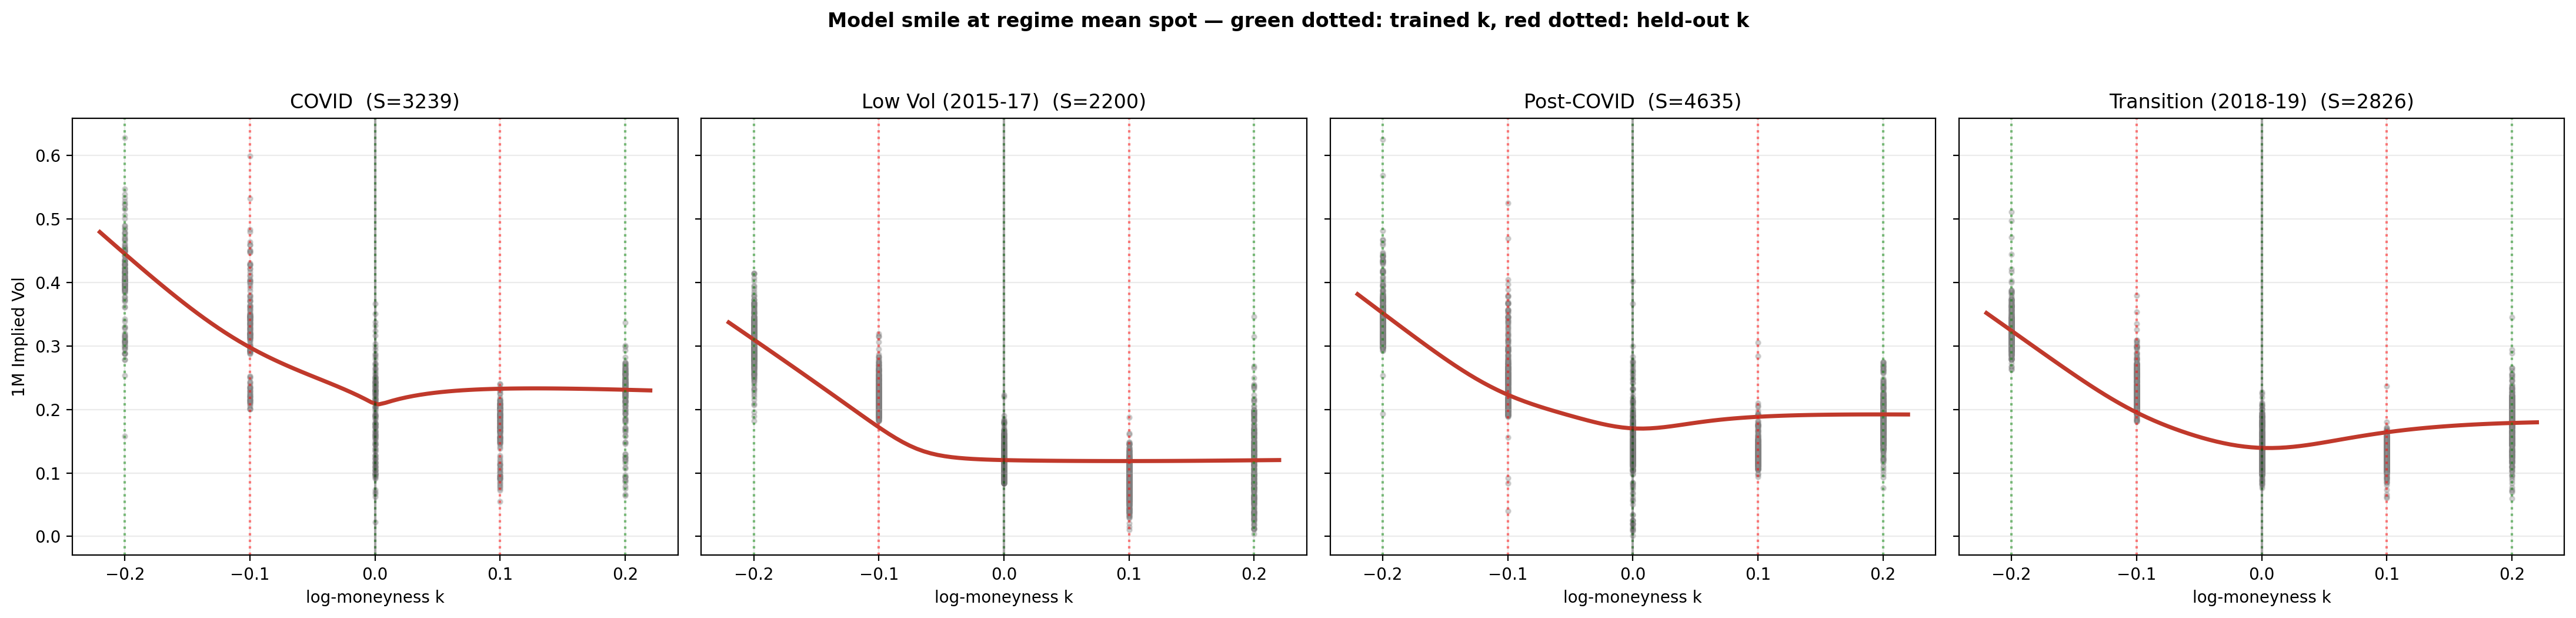
\includegraphics[width=\textwidth]{joint_smile_per_regime.png}
  \caption{Fitted smile per regime, evaluated on a log-moneyness grid $k \in [-0.22, 0.22]$ at the regime-mean spot, overlaid on empirical IV at spots within $\pm 10\%$ of $\bar S_{\mathcal R}$. Green dotted verticals: training strikes $k \in \{\pm 0.20, 0\}$. Red dotted: held-out $k \in \{\pm 0.10\}$.}
  \label{fig:joint_smile}
\end{figure}

\begin{figure}[htbp]
  \centering
  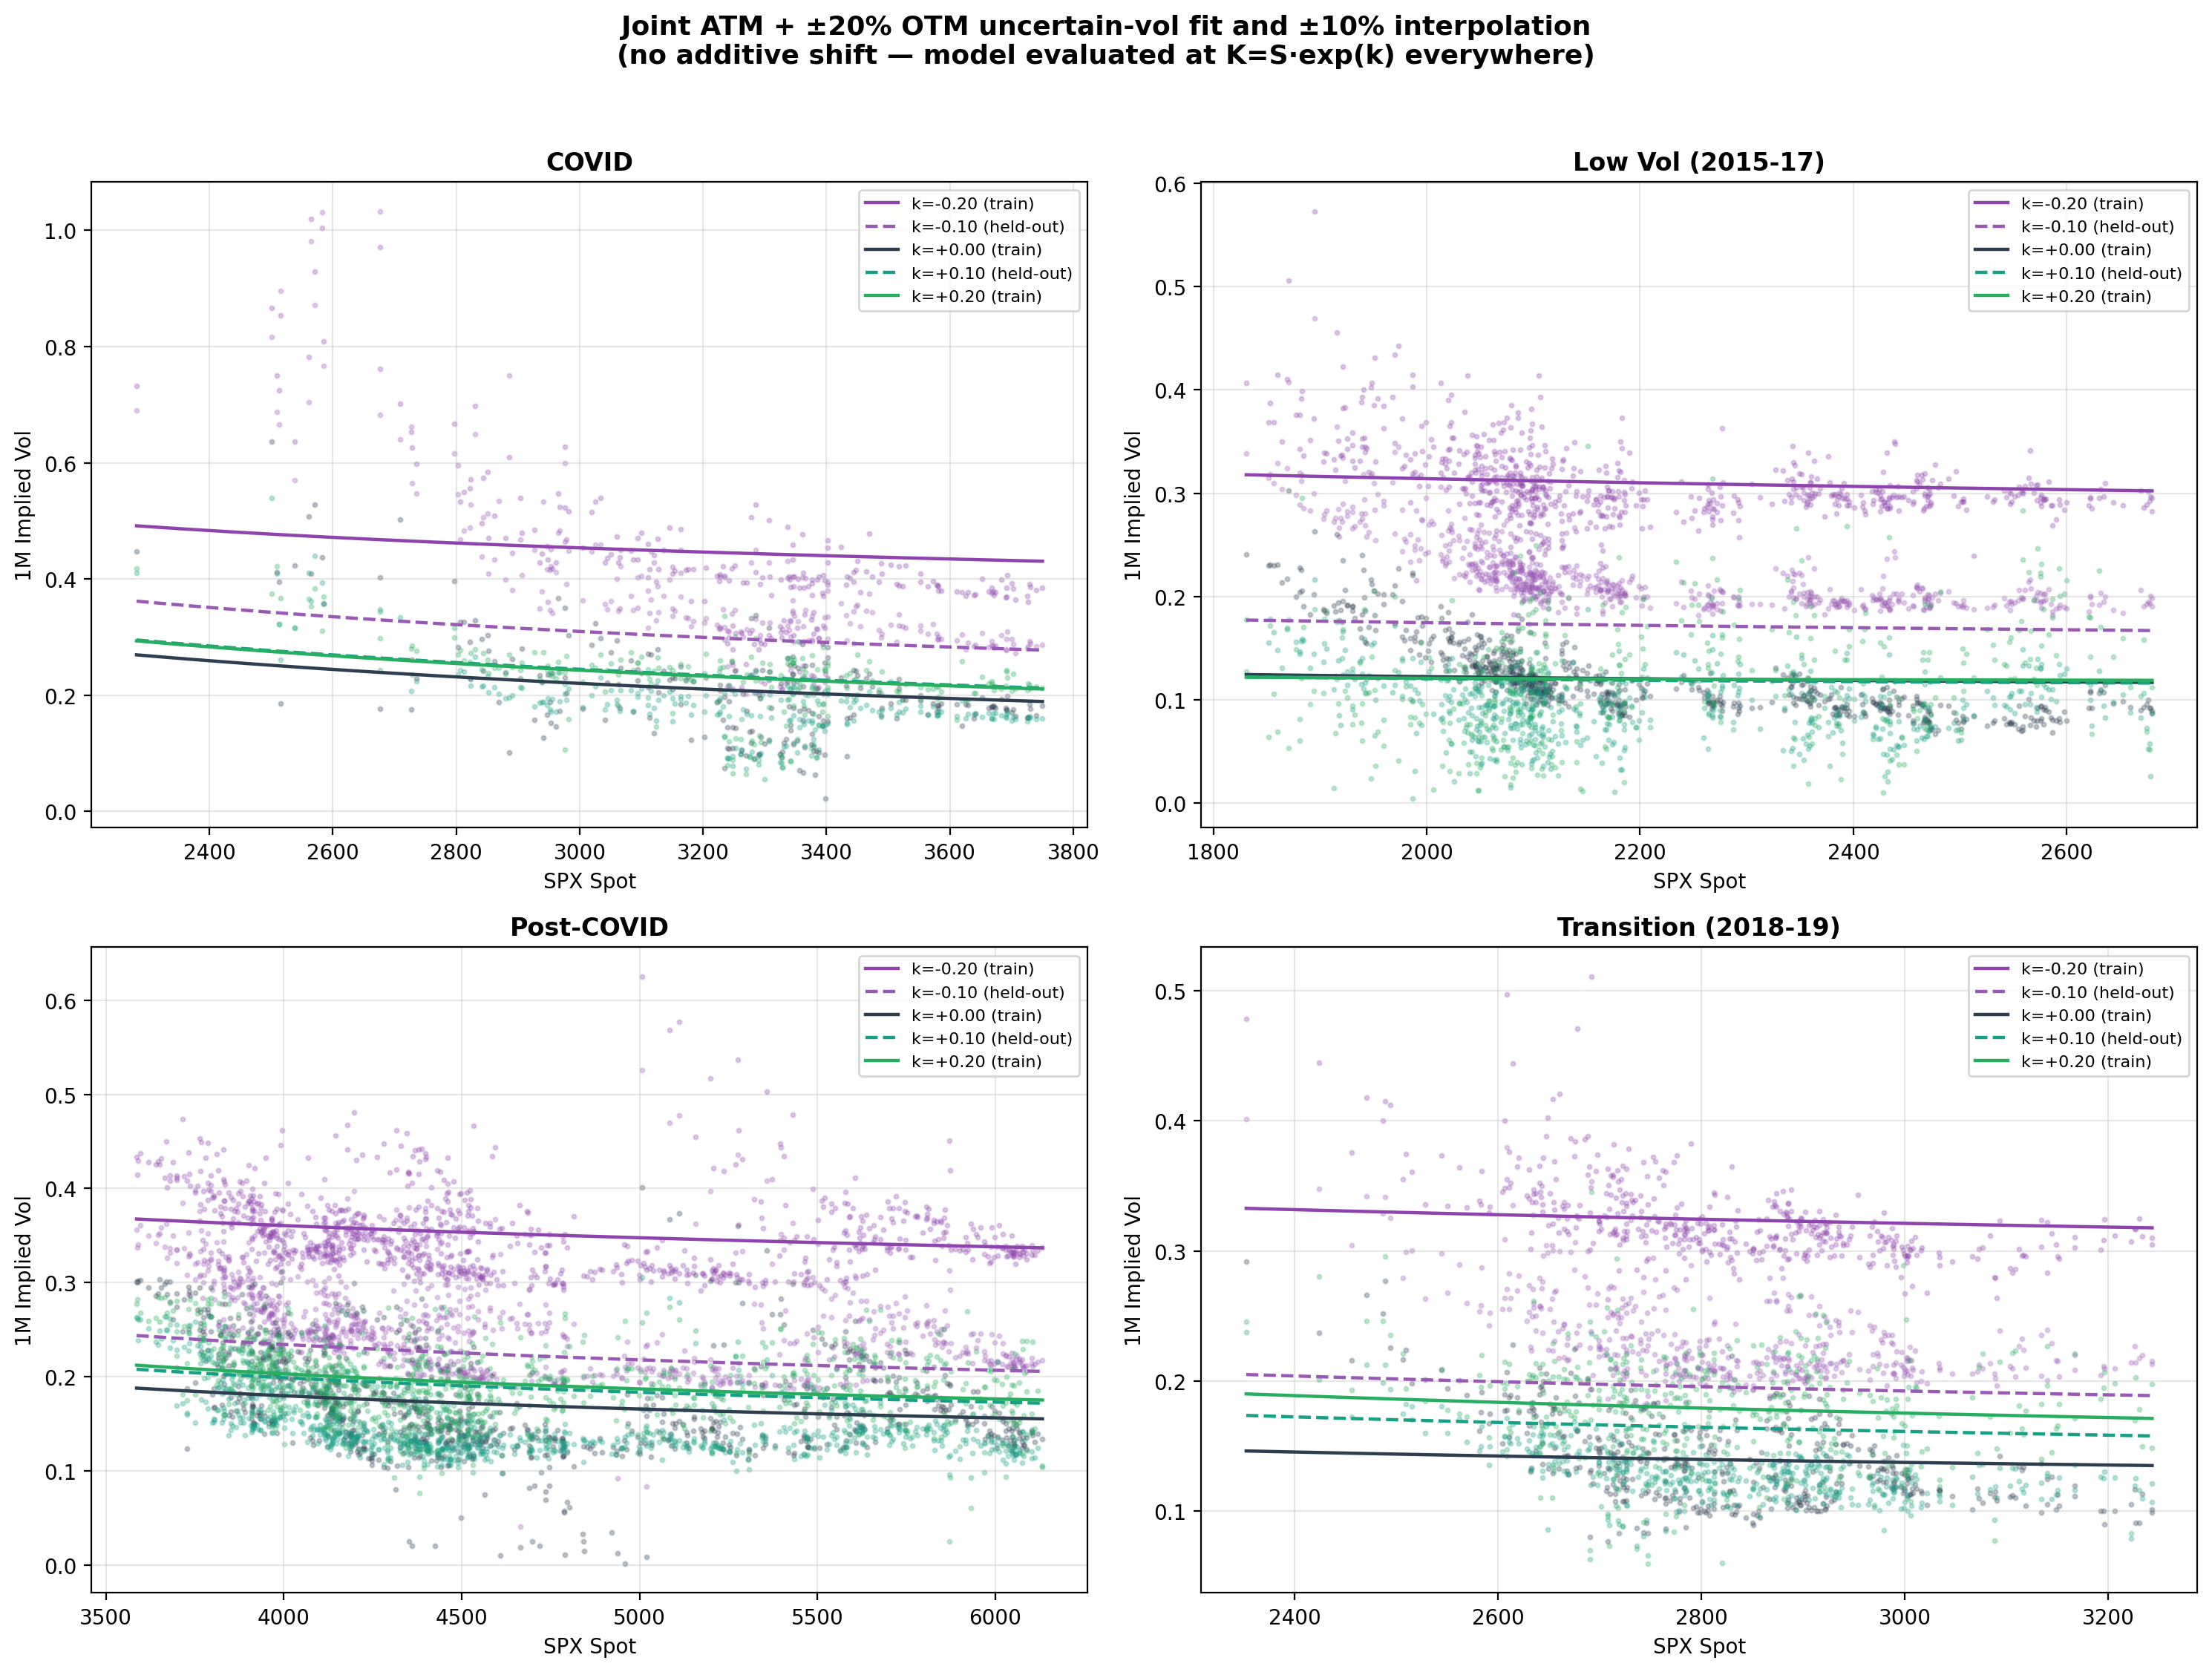
\includegraphics[width=\textwidth]{joint_fit_interpolation.png}
  \caption{Joint calibration: empirical IV (scatter) vs fitted model (curves) at all five moneyness levels. Solid curves are training strikes $k \in \{-0.20, 0, +0.20\}$; dashed curves are the held-out strikes $k \in \{-0.10, +0.10\}$ used only to test interpolation.}
  \label{fig:joint_interp}
\end{figure}

\subsection{The Interpolation Test}

Because $k = \pm 0.10$ is never shown to the optimiser, the quality of the model curve at those strikes is a clean out-of-fit diagnostic. Figure~\ref{fig:joint_interp} shows that the dashed $k = \pm 0.10$ curves land qualitatively near the $\pm 0.10$ scatter in every regime; quantitatively, however, there is a systematic \emph{asymmetric} residual. Table~\ref{tab:joint_bias} reports the mean $(\text{model}-\text{data})$ bias; Table~\ref{tab:joint_rmse} reports the RMSE.

\begin{table}[htbp]
\centering
\caption{Interpolation bias ($\text{model}-\text{data}$, in IV points) by regime and moneyness. Columns $k=\pm 0.10$ are held-out.}
\label{tab:joint_bias}
\small
\begin{tabular}{lccccc}
\toprule
Regime & $k=-0.20$ & $k=-0.10$ & $k=0$ & $k=+0.10$ & $k=+0.20$ \\
\midrule
COVID & $+0.007$ & $\mathbf{-0.066}$ & $+0.001$ & $\mathbf{+0.049}$ & $+0.006$ \\
Low Vol (2015--17) & $+0.001$ & $-0.049$ & $-0.001$ & $+0.025$ & $+0.001$ \\
Transition (2018--19) & $+0.001$ & $-0.035$ & $+0.000$ & $+0.035$ & $+0.000$ \\
Post-COVID & $+0.001$ & $-0.029$ & $+0.000$ & $+0.042$ & $+0.000$ \\
\bottomrule
\end{tabular}
\end{table}

\begin{table}[htbp]
\centering
\caption{Per-strike RMSE by regime. Columns $k=\pm 0.10$ are held-out (interpolation).}
\label{tab:joint_rmse}
\small
\begin{tabular}{lccccc}
\toprule
Regime & $k=-0.20$ & $k=-0.10$ & $k=0$ & $k=+0.10$ & $k=+0.20$ \\
\midrule
COVID & $0.120$ & $0.147$ & $0.077$ & $0.073$ & $0.052$ \\
Low Vol (2015--17) & $0.036$ & $0.059$ & $0.033$ & $0.039$ & $0.058$ \\
Transition (2018--19) & $0.030$ & $0.046$ & $0.032$ & $0.040$ & $0.038$ \\
Post-COVID & $0.039$ & $0.053$ & $0.051$ & $0.051$ & $0.034$ \\
\bottomrule
\end{tabular}
\end{table}

Two regularities stand out:
\begin{enumerate}
  \item \textbf{Asymmetric bias at the held-out strikes.} In every regime the model \emph{underprices} the $k=-0.10$ OTM-put IV (bias $-0.029$ to $-0.066$) and \emph{overprices} the $k=+0.10$ OTM-call IV (bias $+0.025$ to $+0.049$). The sign pattern is universal; the magnitudes are largest for COVID, which is also the worst-fit regime overall. This is the signature of a smile that is too symmetric/linear between the trained strikes: the curvature that empirically lifts the put wing and depresses the call wing at intermediate moneyness is not reproduced by a three-state displaced-diffusion mixture.
  \item \textbf{Trained strikes are well calibrated.} Bias at the trained $k = \{-0.20, 0, +0.20\}$ is within $\pm 0.007$ in every regime, and RMSE there is small relative to the held-out columns. The loss is doing its job where it is given the chance to; the residual is genuinely about between-strike curvature, not about level.
\end{enumerate}

\begin{figure}[htbp]
  \centering
  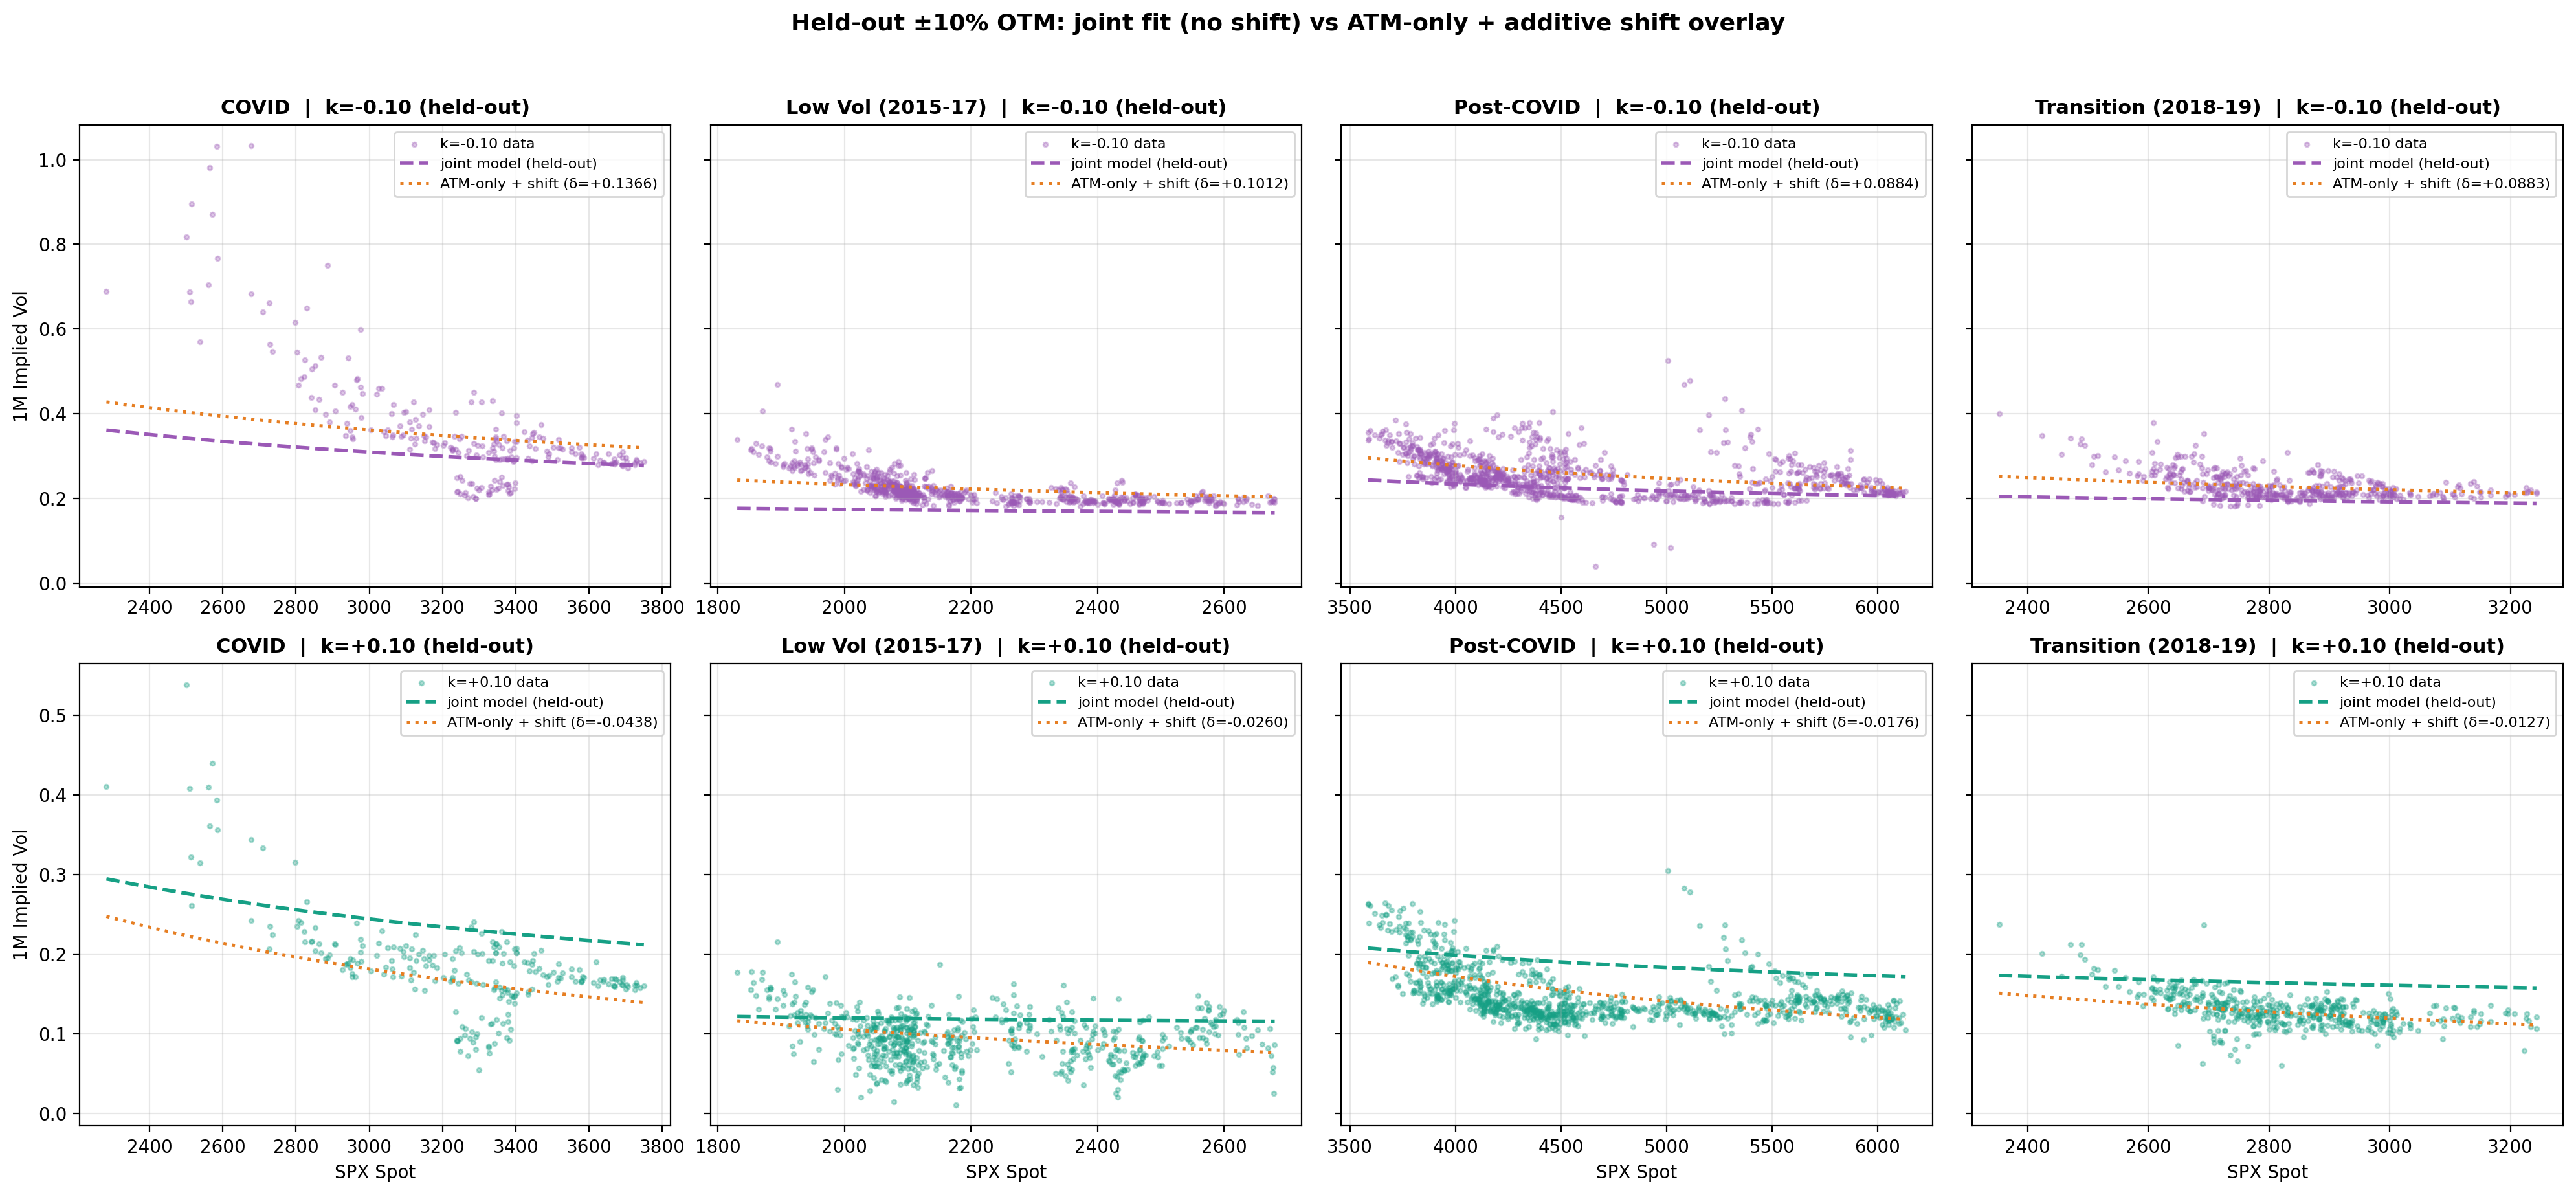
\includegraphics[width=\textwidth]{held_out_interp_closeup.png}
  \caption{Interpolation close-up at the held-out strikes. Top row: $k=-0.10$; bottom row: $k=+0.10$. Dashed curve is the joint-model interpolated IV (no shift); dotted curve is the ATM-only backbone with the additive shift $\delta_k$ applied for comparison. The shift is exact on the mean by construction; the joint curve is not, but is a genuine smile prediction.}
  \label{fig:joint_closeup}
\end{figure}

\subsection{Comparison with the ATM-Only Backbone}

Figure~\ref{fig:joint_vs_atm} overlays the joint-fit ATM backbone ($k=0$ curve) on the ATM-only backbone of Section~\ref{sec:robust_additive}. The two curves coincide almost exactly: adding OTM information has not reshaped the backbone, confirming that the ATM level was already well-identified by ATM data. The OTM degrees of freedom went into the smile shape, not the backbone---exactly as one would hope.

\begin{figure}[htbp]
  \centering
  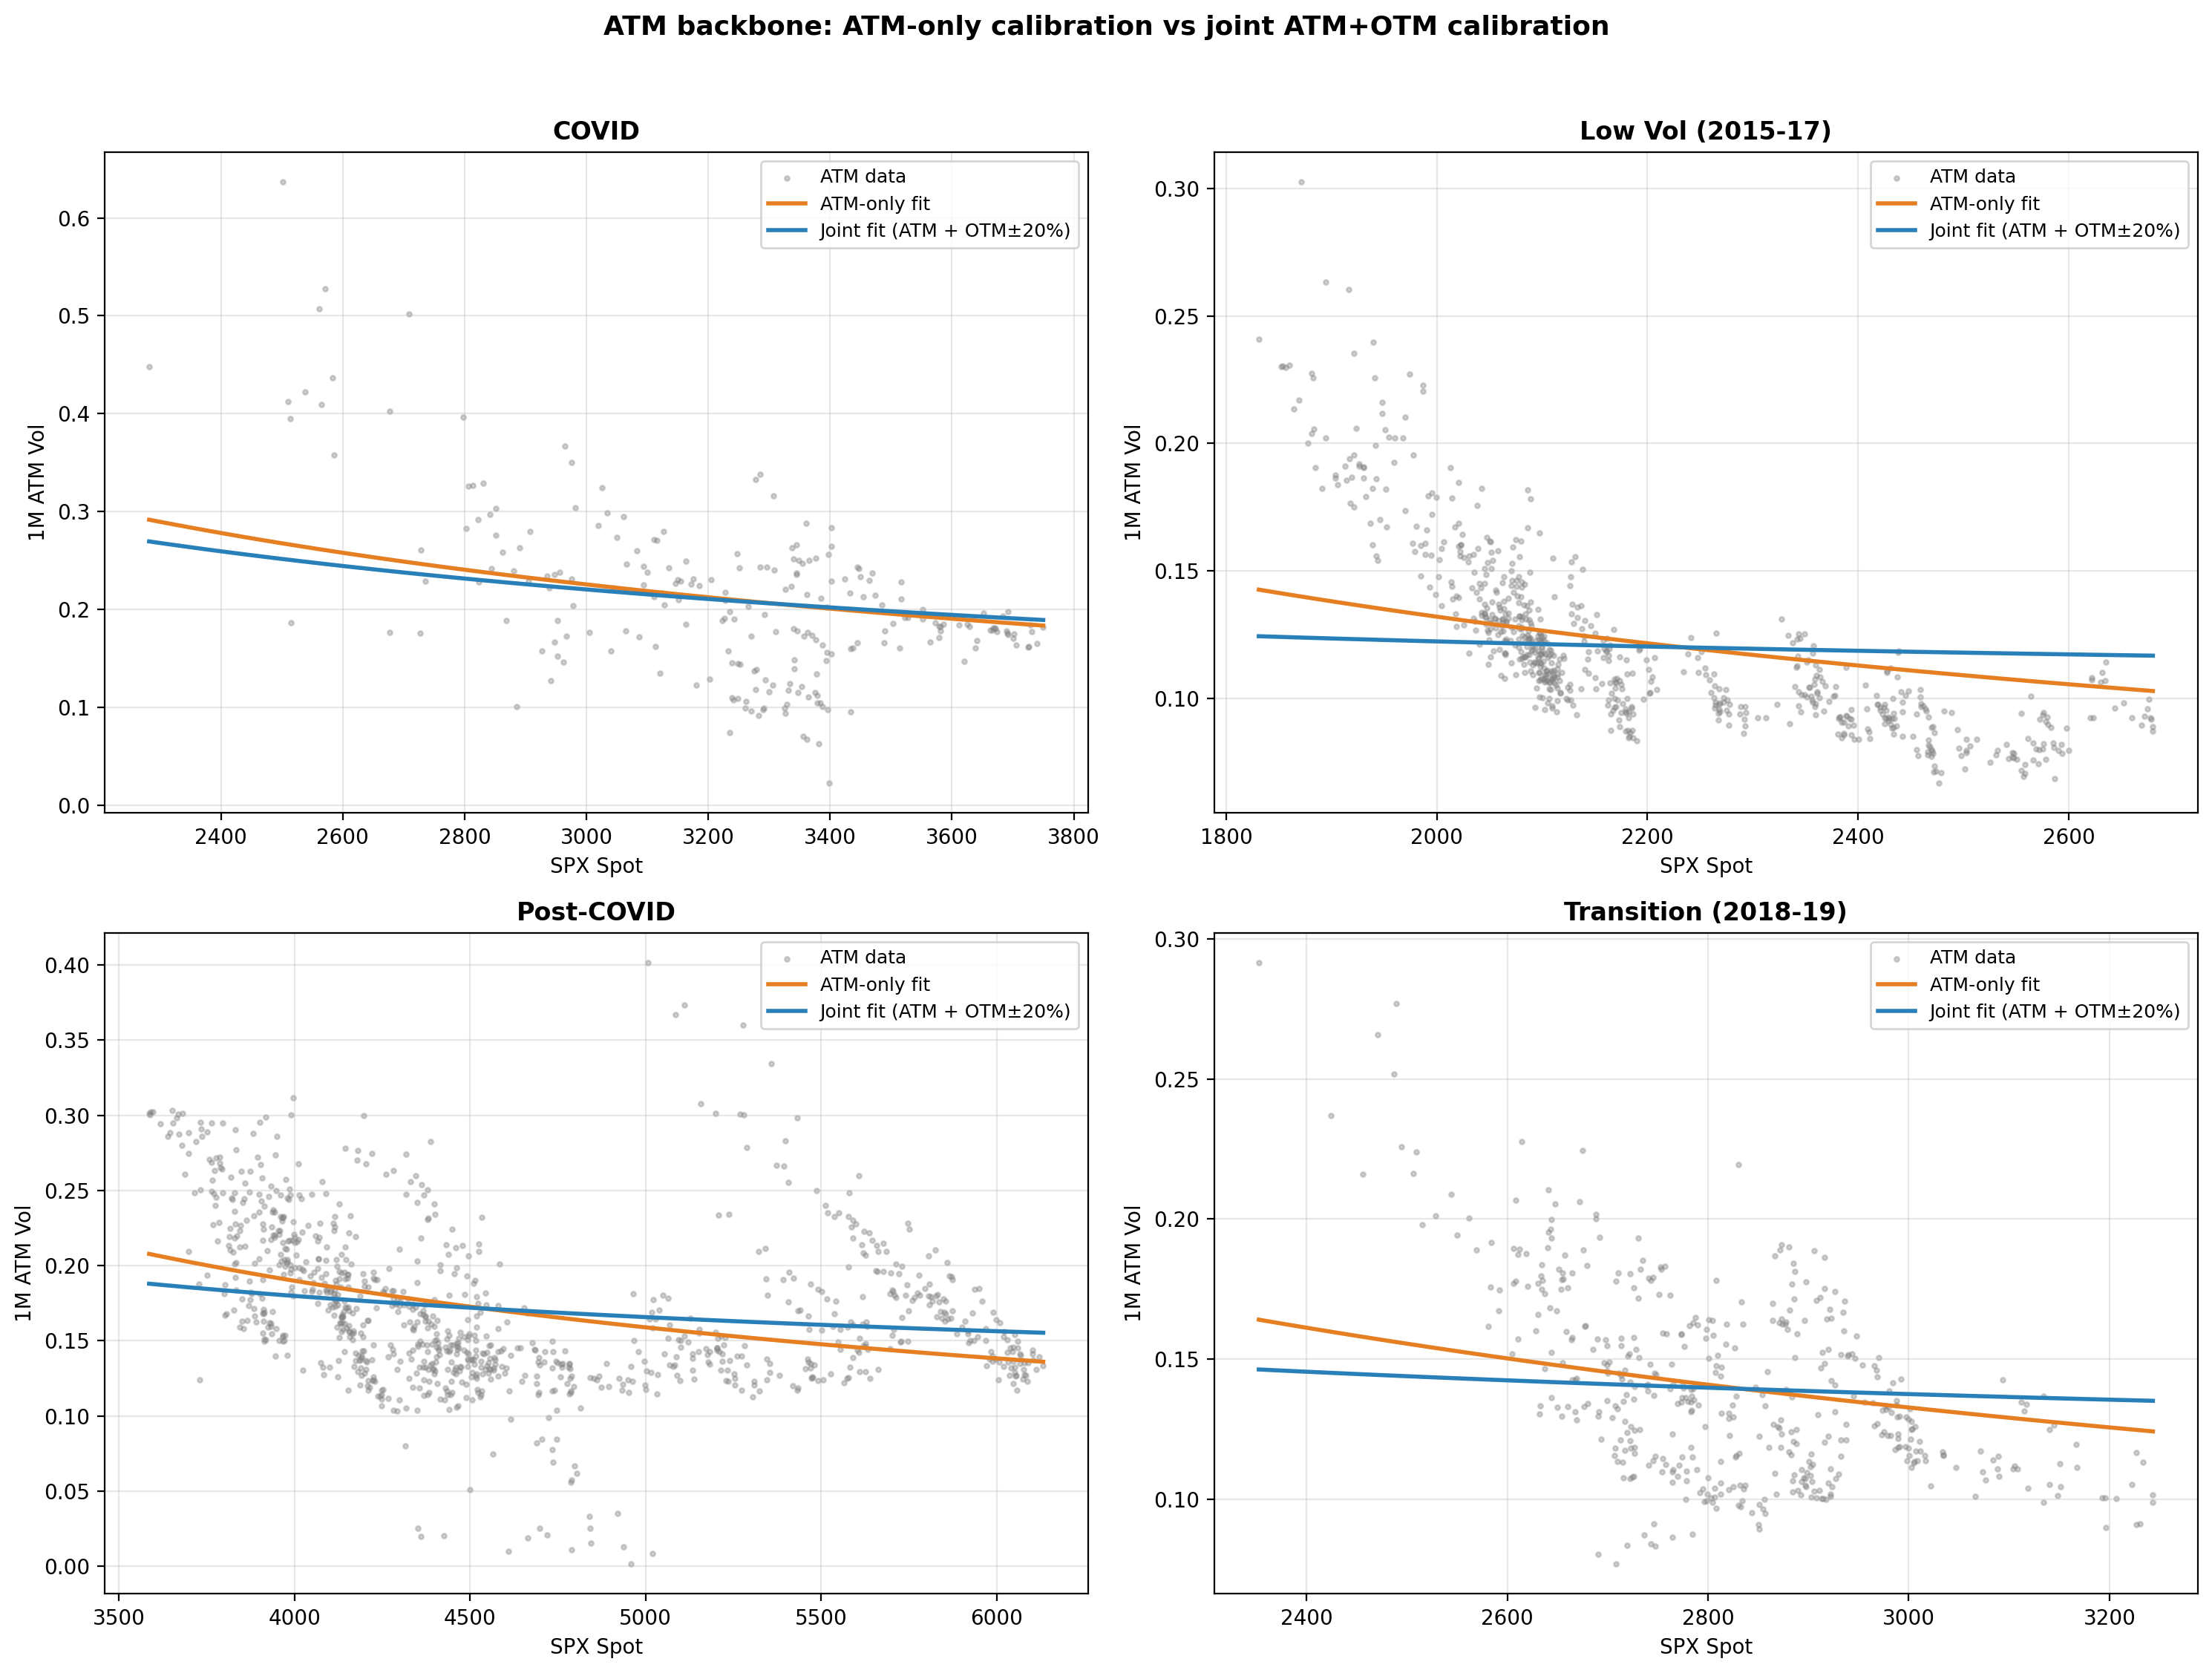
\includegraphics[width=\textwidth]{joint_vs_atm_only_backbone.png}
  \caption{ATM ($k=0$) backbone: joint calibration (blue) vs ATM-only calibration (orange), overlaid on the ATM scatter. The ATM shape is essentially unchanged by the addition of OTM data; the OTM information went into the smile shape, not the backbone.}
  \label{fig:joint_vs_atm}
\end{figure}

\begin{figure}[htbp]
  \centering
  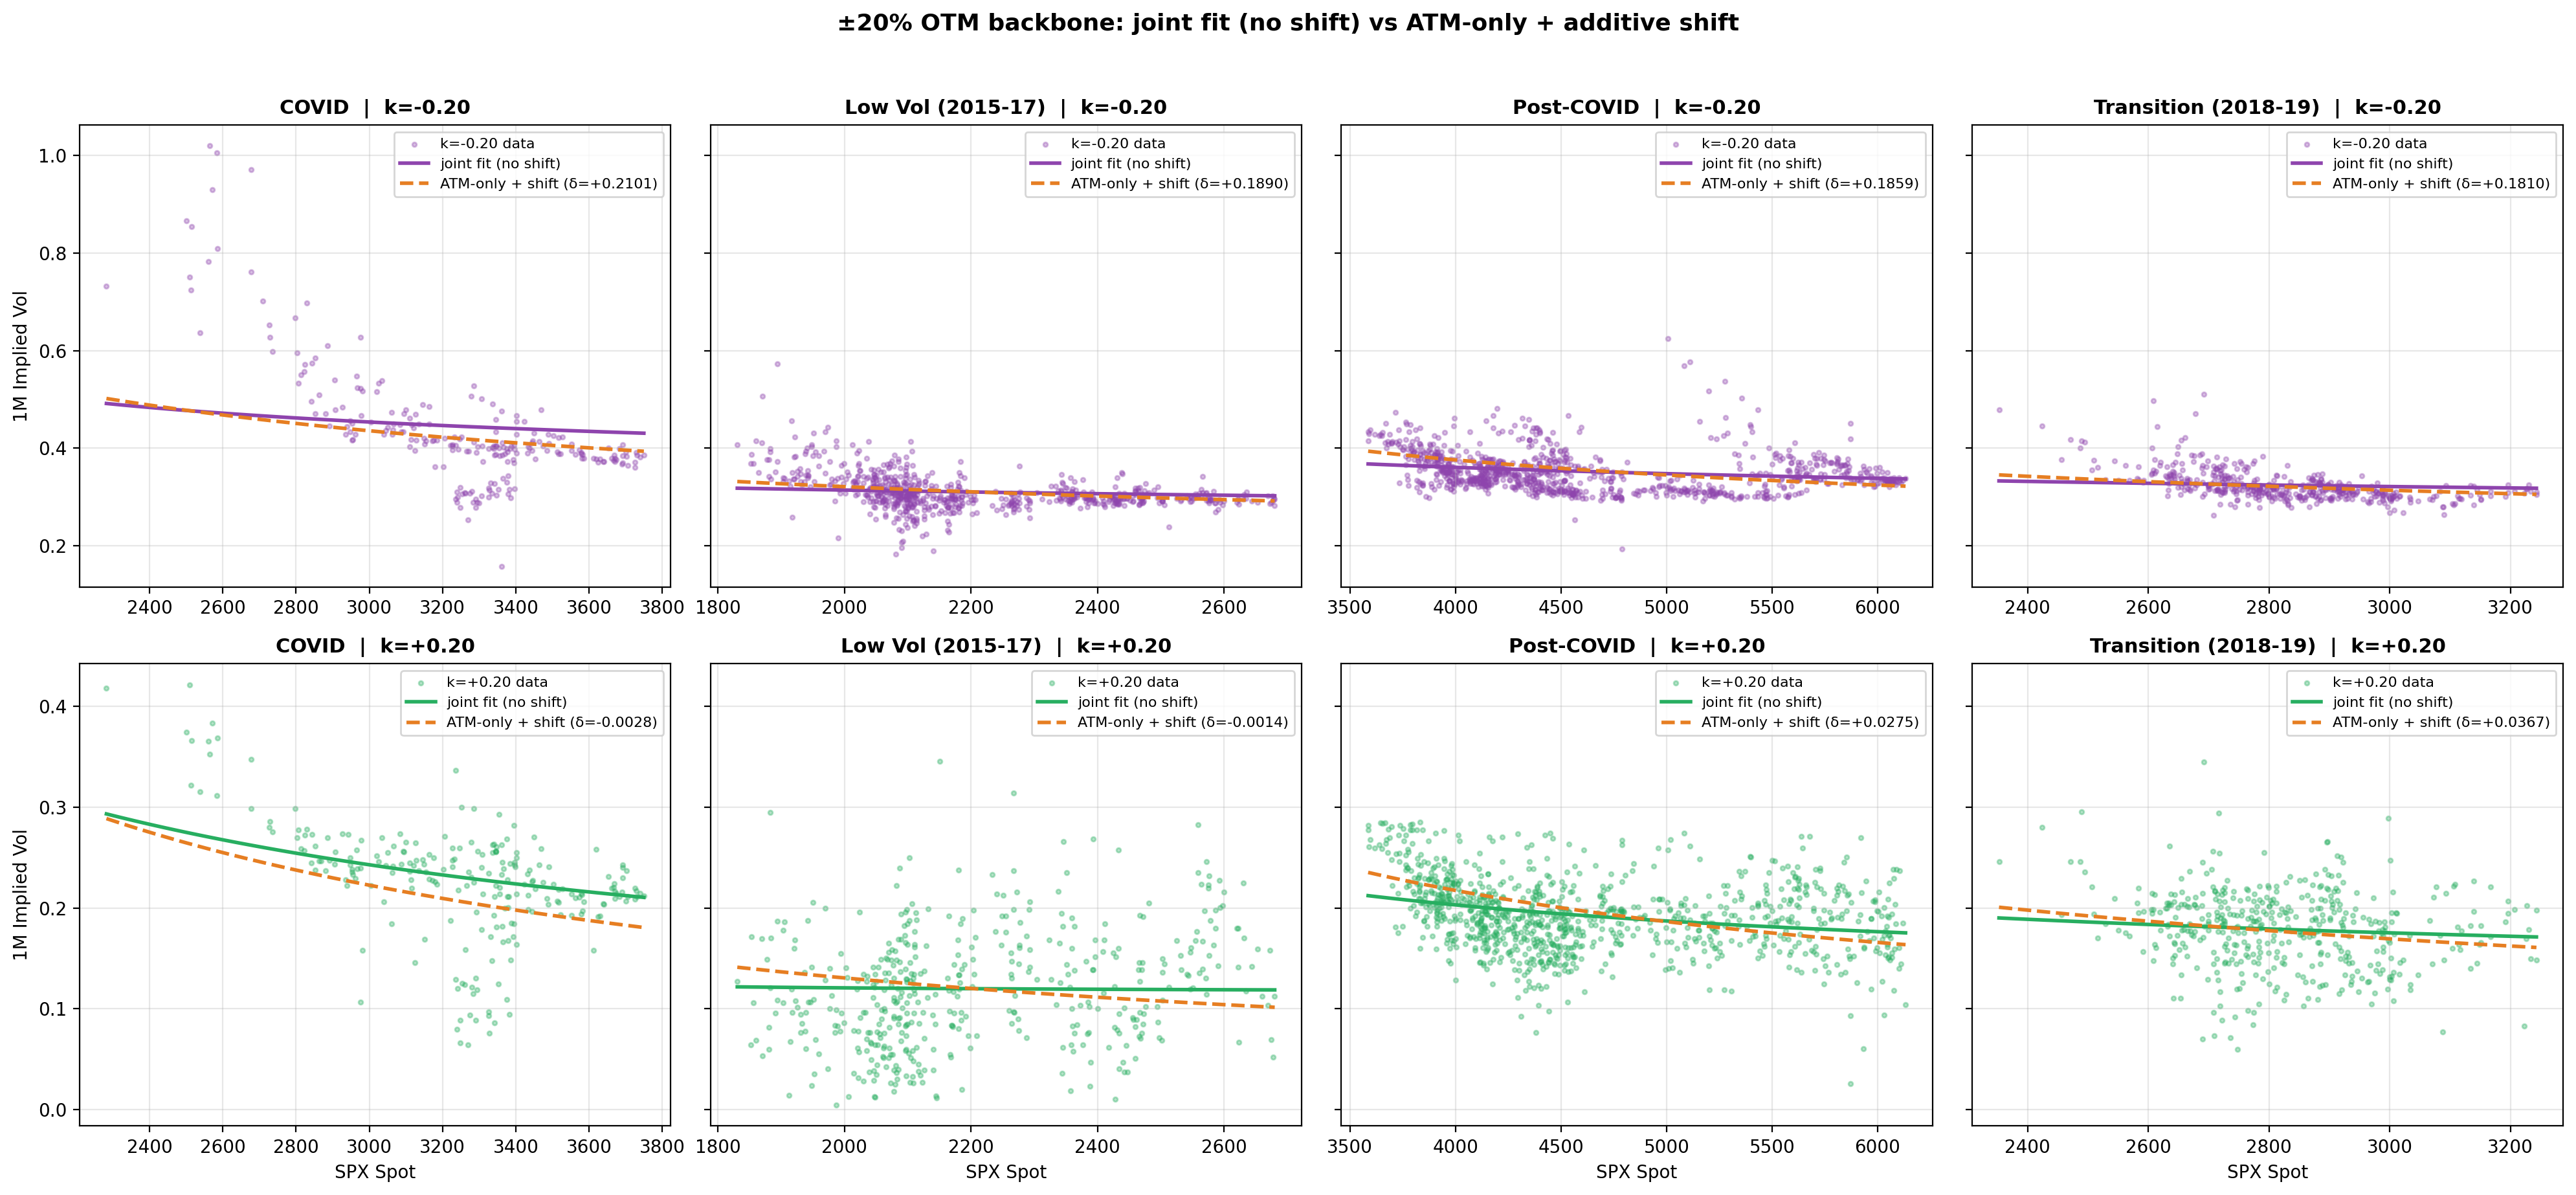
\includegraphics[width=\textwidth]{pm20_joint_vs_atm_shift.png}
  \caption{Trained OTM tails ($k=\pm 0.20$), joint fit vs ATM-only with additive shift. The solid joint-model curve reproduces the trained-tail data \emph{without} any shift; the dashed overlay is the ATM-only backbone with the empirical $\delta_k$ applied---the two are visually indistinguishable at the trained strikes, but only the joint curve is a smile prediction.}
  \label{fig:joint_pm20}
\end{figure}

\subsection{Structural Findings}

\paragraph{Endogenous smile, retired shift.} The joint fit reproduces the $k = \pm 0.20$ IV directly from $K = S\,e^{k}$ with no shift; Figure~\ref{fig:joint_pm20} shows the joint curve tracking the trained-tail data as well as the explicit additive-shift overlay. This is the central methodological claim of the paper: with the right loss, the mixture's $\beta$-driven skew is sufficient to retire the ad hoc shift on the trained strikes.

\paragraph{One bound $\beta$ per regime.} Each regime pins exactly one of the three $\beta$ to the upper bound $0.95$. This suggests the three-state mixture has one redundant state for SPX: a two-state displaced-diffusion mixture with an additional curvature degree of freedom (or a four-state mixture that allows a genuine intermediate skew state) is the parsimonious next step.

\paragraph{COVID is the stress test.} The COVID RMSE at $k=-0.10$ is $0.147$---roughly three times the RMSE in calmer regimes. The COVID smile is too steep and too curved for the symmetric three-state mixture; the optimiser responds by collapsing $\sigma_{\ln,1}$ to the floor and seating $\beta_2 \approx \beta_3 \approx 0.32$ on two near-identical states (a near-degenerate pair). This is the regime where the asymmetric interpolation bias is most visible.

\paragraph{ATM backbone stability.} The ATM backbone is essentially unchanged by the addition of OTM data (Figure~\ref{fig:joint_vs_atm}). The OTM signal constrains the smile shape without distorting the backbone, which we read as evidence that the joint loss is well-conditioned: the two pieces of information (level at $k=0$, curvature at $|k|=0.20$) act on different parameter subspaces.


\section{Robustness Checks: Alternative OTM Extensions}
\label{sec:robust}

Before arriving at the joint calibration of Section~\ref{sec:joint}, we explored three simpler ways of extending the ATM backbone to OTM strikes. Each is documented below as a robustness check: we describe the method, the reason it was tried, the results, and why it was ultimately abandoned in favour of the joint approach. The thread running through all three is that each attempts to \emph{patch} the dead-state problem after the fact---by shifting (Section~\ref{sec:robust_additive}), by pinning $\sigma$ to percentiles (Section~\ref{sec:robust_percentile}), or by changing parameterisation (Section~\ref{sec:robust_pricelevel})---and each either relocates the degeneracy or fails numerically. Only the joint loss addresses the cause directly.

\subsection{Additive-Shift Extension of the ATM Backbone}
\label{sec:robust_additive}

\paragraph{Method.} The 9-parameter backbone is fitted to ATM data only ($K=S$, $\tau=30/365$, $r=0.02$) via L-BFGS-B with MSE loss and the bounds of Section~\ref{sec:joint}. Two of the three $\sigma_{\ln}$ collapse to the $0.01$ floor in every regime (Table~\ref{tab:params}: states~1 and 2 are ``dead''). The model's intrinsic $\beta$-driven skew is too weak to reproduce the empirical OTM put premium, so OTM IV is constructed as an additive shift:
\begin{equation}
  \text{IV}_{\text{OTM}}(S,k) = \text{IV}_{\text{ATM}}^{\text{model}}(S) + \delta_k,
  \qquad
  \delta_k = \overline{\text{IV}_k^{\text{obs}}} - \overline{\text{IV}_{\text{ATM}}^{\text{model}}}.
\end{equation}
That is, one scalar per (regime, moneyness) pair: the mean observed OTM IV minus the mean model ATM IV over the regime's spot range. The ATM \emph{shape} (negative vol/spot slope, convexity) is preserved exactly; only the level is moved.

\paragraph{Why an additive shift rather than proportional or affine.} Three candidates were considered: additive ($+\delta_k$), proportional ($\lambda_k\,\text{IV}_{\text{ATM}}$), and the affine generalisation ($\alpha_k+\beta_k\,\text{IV}_{\text{ATM}}$). Informal regressions of OTM observed IV on ATM model IV produce slopes near unity, $\beta_k \approx 1$, across moneyness levels, under which the affine model collapses to the additive shift: the OTM--ATM co-movement is approximately parallel, not proportional. The proportional shift distorts curvature (it scales the backbone, amplifying peaks and compressing troughs) and introduces an unwanted slope modifier once $\beta_k \approx 1$, so it is dominated by the additive shift under the empirical evidence.

\paragraph{Results.} Table~\ref{tab:params} reports the ATM-only fit (the baseline against which Section~\ref{sec:joint} is compared) and Table~\ref{tab:shifts} reports the additive shifts $\delta_k$. As expected, $\delta_k$ is positive and large for OTM puts (the skew premium, peaking at $k=-0.20$: $\delta \in [0.18, 0.21]$) and small or negative for OTM calls ($\delta \in [-0.04, +0.04]$ at $k \in \{+0.10,+0.20\}$).

\begin{table}[htbp]
\centering
\caption{Baseline ATM-only three-state displaced-diffusion fit (fitted parameters, MSE loss). Repeated here as the reference for the joint calibration and the additive shift.}
\label{tab:params}
\small
\begin{tabular}{lcccc}
\toprule
& Low Vol & Transition & COVID & Post-COVID \\
& (2015--17) & (2018--19) & (2020) & (2021--25) \\
\midrule
$w_1$ & 0.387 & 0.384 & 0.254 & 0.377 \\
$w_2$ & 0.340 & 0.338 & 0.261 & 0.333 \\
$w_3$ & 0.272 & 0.278 & 0.486 & 0.291 \\
\midrule
$\beta_1$ & 0.895 & 0.884 & 0.135 & 0.912 \\
$\beta_2$ & 0.901 & 0.891 & 0.100 & 0.872 \\
$\beta_3$ & 0.100 & 0.100 & 0.100 & 0.184 \\
\midrule
$\sigma_{\ln,1}$ & 0.010 & 0.010 & 0.010 & 0.010 \\
$\sigma_{\ln,2}$ & 0.010 & 0.010 & 0.010 & 0.010 \\
$\sigma_{\ln,3}$ & 0.343 & 0.401 & 0.236 & 0.517 \\
\midrule
ATM MSE & 0.000795 & 0.000907 & 0.005632 & 0.002463 \\
$n$ & 705 & 471 & 234 & 995 \\
\bottomrule
\end{tabular}
\end{table}

\begin{table}[htbp]
\centering
\caption{Additive shifts $\delta_k$ (mean observed OTM IV $-$ mean model ATM IV) by regime and moneyness.}
\label{tab:shifts}
\begin{tabular}{lccccc}
\toprule
Regime & $k=-20\%$ & $k=-10\%$ & $k=0\%$ & $k=+10\%$ & $k=+20\%$ \\
\midrule
COVID & $+0.210$ & $+0.137$ & $0.000$ & $-0.044$ & $-0.003$ \\
Low Vol (2015--17) & $+0.189$ & $+0.101$ & $0.000$ & $-0.026$ & $-0.001$ \\
Post-COVID & $+0.186$ & $+0.088$ & $0.000$ & $-0.018$ & $+0.028$ \\
Transition (2018--19) & $+0.181$ & $+0.088$ & $0.000$ & $-0.013$ & $+0.037$ \\
\bottomrule
\end{tabular}
\end{table}

\begin{figure}[htbp]
  \centering
  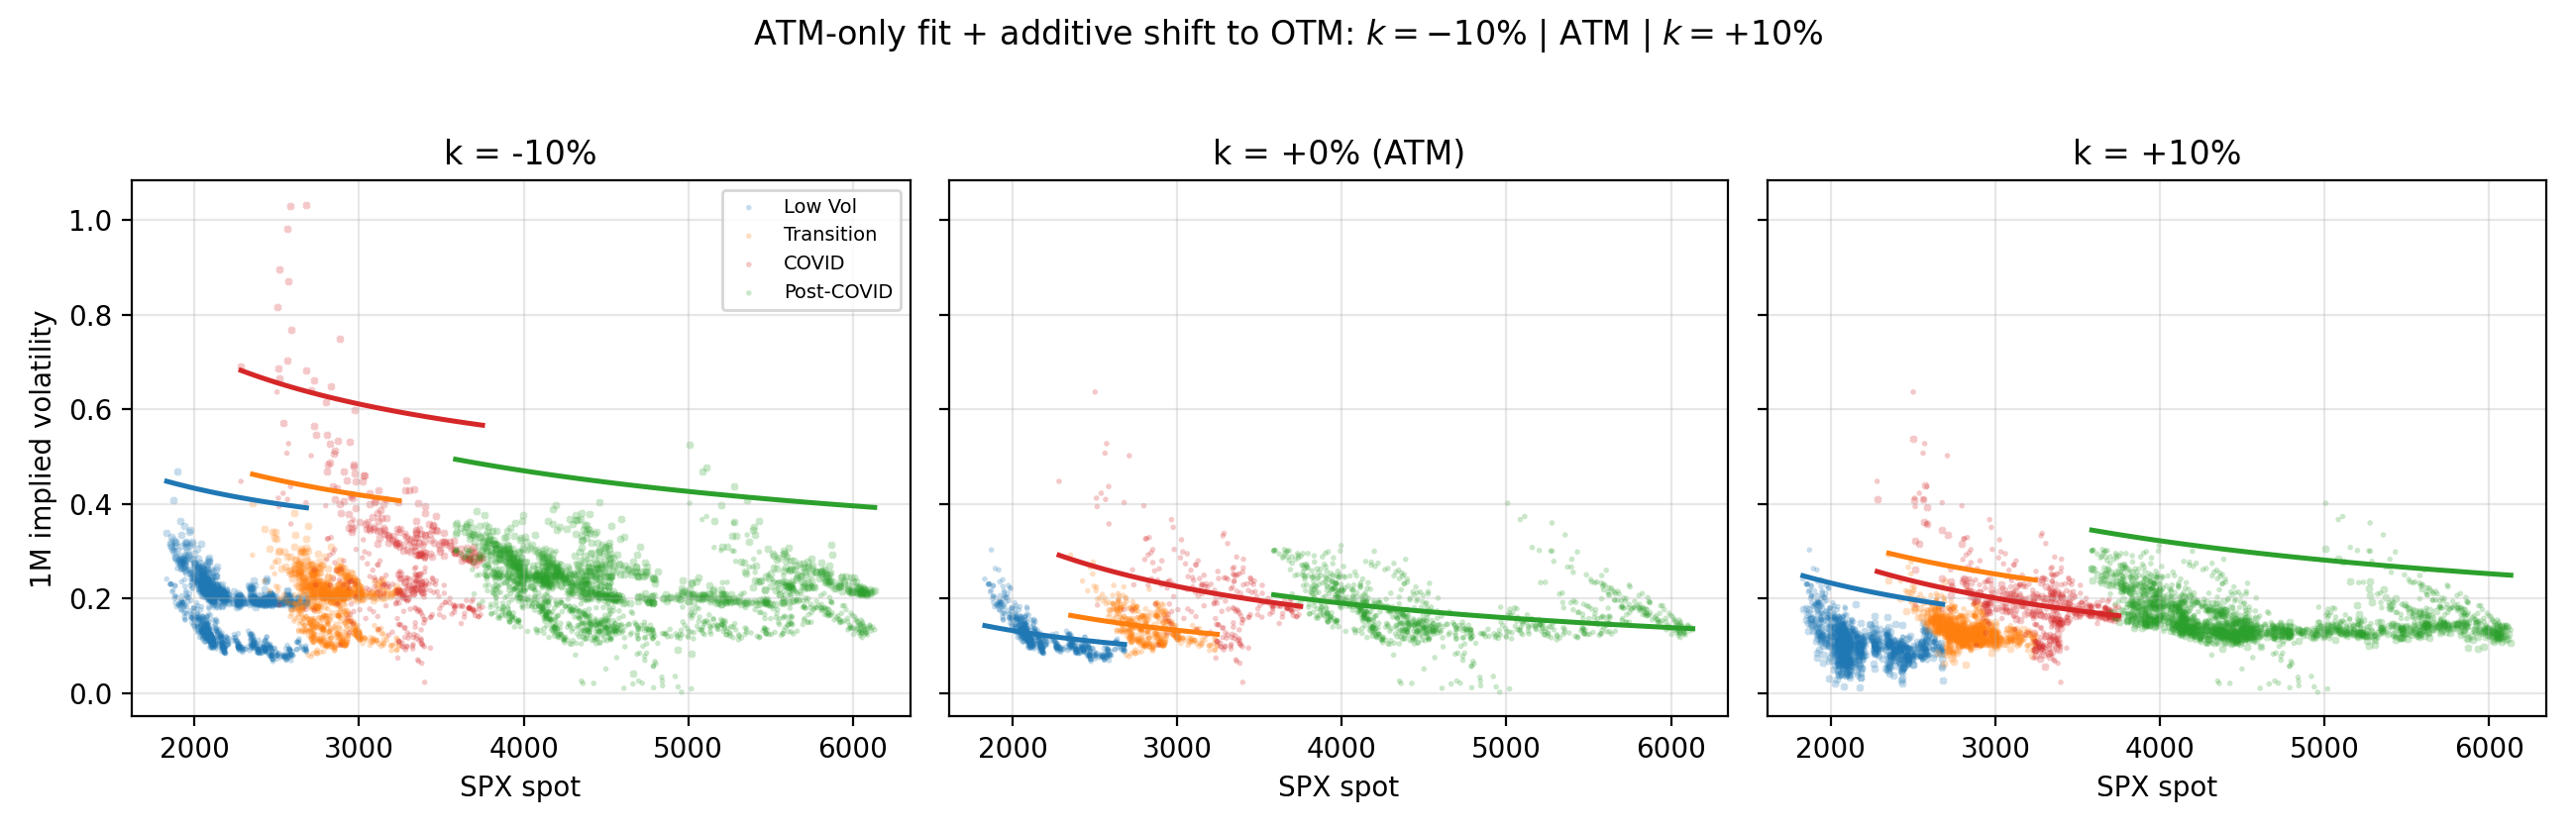
\includegraphics[width=\textwidth]{robust_additive_shift_triptych.png}
  \caption{Additive-shift extension: observed IV (dots) and shifted-backbone curves for $k=-10\%$ (OTM put), $k=0\%$ (ATM), and $k=+10\%$ (OTM call). The ATM shape is preserved; only the level moves by $\delta_k$.}
  \label{fig:otm_triptych}
\end{figure}

\begin{figure}[htbp]
  \centering
  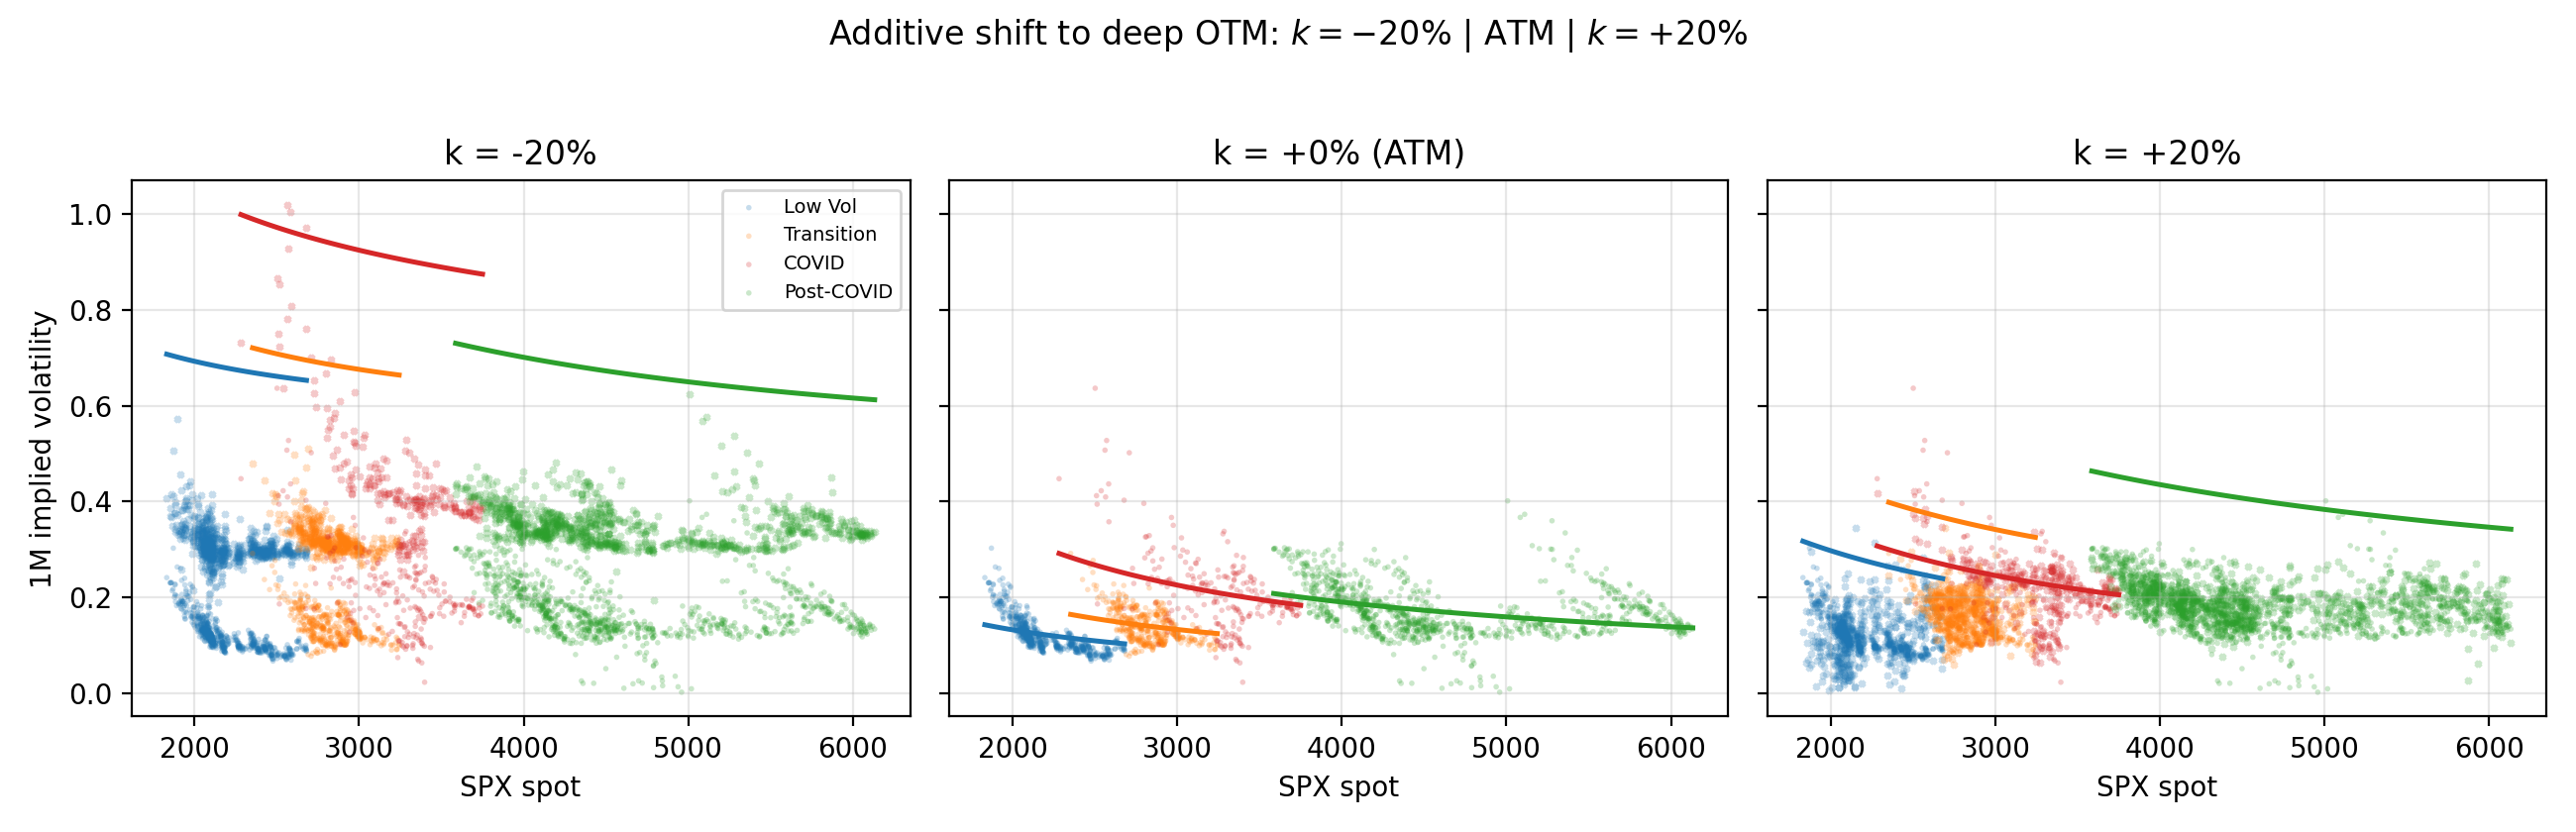
\includegraphics[width=\textwidth]{robust_additive_shift_deep.png}
  \caption{Additive-shift extension at the deep OTM wings: $k=-20\%$, ATM, $k=+20\%$. The deep-OTM put shift is the largest correction and is consistent in size across regimes.}
  \label{fig:otm_deep}
\end{figure}

\paragraph{Why it was abandoned.} The additive shift is exactly correct on the regime-mean by construction, but it is not a smile prediction: it carries no information about curvature between anchor strikes, it assumes the OTM--ATM spread is constant across the spot range (the skew actually flattens at very high spot within a regime), and its $\beta_k \approx 1$ justification rests on informal regressions rather than a held-out test. Its role in the paper is now as the \emph{baseline against which the joint calibration of Section~\ref{sec:joint} is measured}: Figure~\ref{fig:joint_closeup} shows that the joint-model interpolation at $k=\pm 0.10$ competes with the shift \emph{despite} the shift being exact-on-mean, and Figure~\ref{fig:joint_pm20} shows the joint model matches the trained tails without any shift at all. The shift is retained as a benchmark; it is not the production methodology.

\subsection{Percentile-Pinned $\sigma$ Variants (6-Parameter)}
\label{sec:robust_percentile}

\paragraph{Motivation.} The dead-state problem of Section~\ref{sec:robust_additive} is, at root, a $\sigma$-collapse: two of the three log-volatilities flee to the lower bound, leaving one state with all the variance. The percentile-pinned variant tries to eliminate this collapse \emph{by construction}: per regime, the three $\sigma_{\ln}$ are pinned to the 5th, 50th, and 95th percentiles of the regime's own observed ATM 1M IV series, ordered low--median--high so the $\beta$/$\sigma$ pairing is interpretable. Only six parameters then remain free---the three weight-logits and the three $\beta$---but because all three $\sigma$ are now economically meaningful vols, \emph{no} state can wash out to a near-zero premium, and the mixture should generate a genuine three-state smile at $K \ne S$ that lets OTM IV be read directly off the model rather than via an additive shift.

\begin{table}[htbp]
\centering
\caption{Pinned $\sigma_{\ln}$ values (regime-own ATM IV percentiles) used for both 6p variants.}
\label{tab:pinned_sigma}
\small
\begin{tabular}{lccc}
\toprule
Regime & $p_5$ & $p_{50}$ & $p_{95}$ \\
\midrule
Low Vol (2015--17) & 0.0797 & 0.1139 & 0.1918 \\
Transition (2018--19) & 0.0990 & 0.1334 & 0.1958 \\
COVID & 0.0991 & 0.1913 & 0.3764 \\
Post-COVID & 0.1137 & 0.1615 & 0.2727 \\
\bottomrule
\end{tabular}
\end{table}

The loss is the same ATM-only MSE as in Section~\ref{sec:robust_additive}; OTM is again only a diagnostic. The optimiser is L-BFGS-B with multistart ($N=16$). We tested two $\beta$ regimes:

\begin{itemize}
  \item \textbf{6p:} $\beta \in [0.10, 0.95]$ (the same range as the 9-parameter fit).
  \item \textbf{6p-tight:} $\beta \in [0.50, 0.95]$, capping the displacement leverage $|\sigma_n (1-\beta)/(\sigma_{\ln}\beta)|$ at $\bar S_{\mathcal R}$.
\end{itemize}

\paragraph{Results.} Pinning $\sigma$ does eliminate $\sigma$-collapse. It does not eliminate the degeneracy: the optimiser simply relocates the collapse.

\begin{table}[htbp]
\centering
\caption{Percentile-pinned fits (6p, $\beta \in [0.10,0.95]$): ATM MSE matches the 9p fit, but weights go one-hot on the lowest-$\sigma$ state and $\beta$ drops to the floor.}
\label{tab:6p}
\small
\begin{tabular}{lccccc}
\toprule
Regime & $w$ (softmax) & $\beta$ & ATM MSE (6p) & ATM MSE (9p) & OTM direct RMSE \\
\midrule
Low Vol (2015--17) & $[0.9998,0.0002,0]$ & $[0.169,0.103,0.107]$ & 0.000787 & 0.000795 & 0.135 \\
Transition (2018--19) & $[0.9998,0.0002,0]$ & $[0.169,0.100,0.149]$ & 0.000905 & 0.000907 & 0.131 \\
COVID & $[0.846,0.059,0.094]$ & $[0.100,0.100,0.100]$ & 0.005626 & 0.005632 & 0.125 \\
Post-COVID & $[0.492,0.463,0.045]$ & $[0.257,0.208,0.353]$ & 0.002463 & 0.002463 & 0.080 \\
\bottomrule
\end{tabular}
\end{table}

\begin{itemize}
  \item In Low Vol and Transition the weights go essentially one-hot on the $p_5$ state ($w_1 \approx 0.9998$); the median and $p_{95}$ states are dormant. Pinning $\sigma$ did not activate three states---it gave the optimiser a single well-placed low-$\sigma$ state to dump weight on.
  \item $\beta$ falls to the $0.10$ floor in most states (COVID: all three). With $\beta = 0.10$ the displacement shift inside the pricer is $\bar S_{\mathcal R}\cdot 9$, a $\sim$10$\times$ leverage on the spot scale; the shifted lognormal is then translated far from the spot band over which data is observed, and the smiles returned are \emph{much} wider than observed.
  \item The consequence, quantified as a direct OTM evaluation (no shift): the OTM put IV is \emph{over}-estimated by $+47\%$ to $+87\%$ at $k=-0.20$ across all four regimes. The OTM direct RMSE ($0.08$--$0.13$) exceeds the magnitude of the additive shift it was meant to retire ($0.08$--$0.10$). The ATM fit was recovered at the cost of a wildly over-amplified smile.
\end{itemize}

\begin{figure}[htbp]
  \centering
  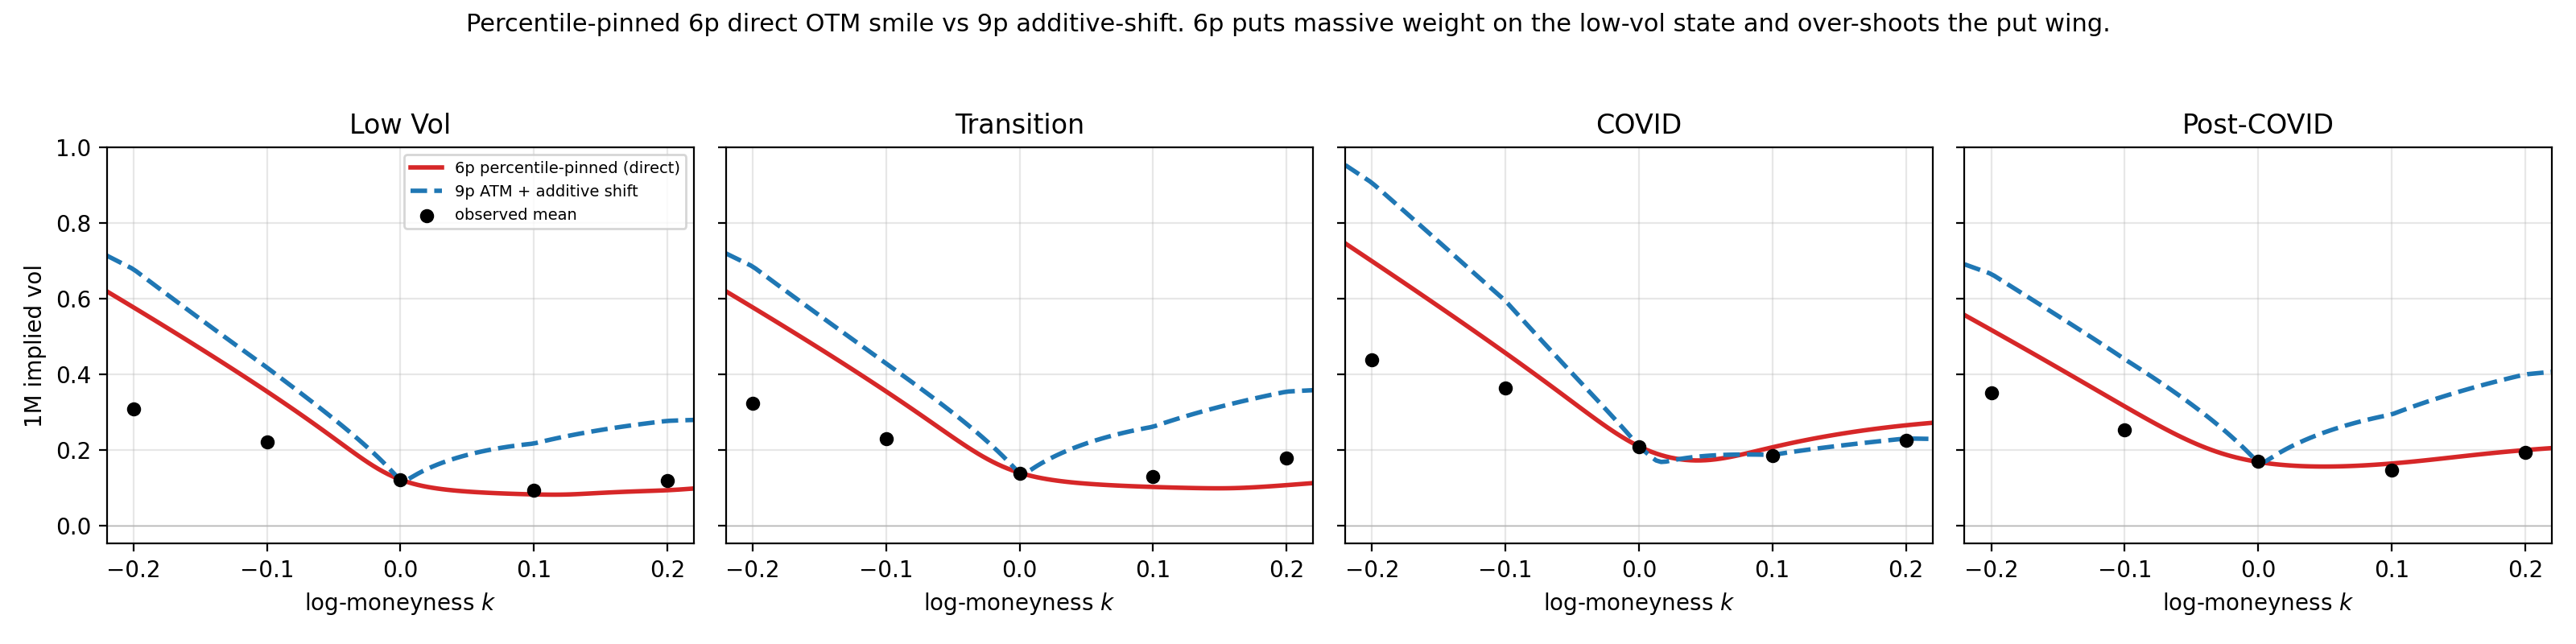
\includegraphics[width=\textwidth]{robust_percentile_6p_overshoot.png}
  \caption{6p percentile-pinned direct OTM smile (red) vs 9p ATM-only with additive shift (blue dashed) at the regime-mean spot. The 6p curve over-shoots the OTM put wing by $+47\%$ to $+87\%$: the collapse has relocated from $\sigma \to \text{floor}$ in 9p to $\text{weights} \to \text{one-hot}$ and $\beta \to \text{floor}$ in 6p.}
  \label{fig:6p_overshoot}
\end{figure}

\paragraph{Tight-$\beta$ variant.} The tight-$\beta$ variant tests the obvious fix---raise the $\beta$ floor to $0.50$. The collapse relocates a second time: $\beta$ pins to the \emph{new} floor $(0.50,0.50,0.50)$ in every regime, the weights spread to a compensating $\approx 0.50/0.25/0.25$, and the ATM MSE \emph{degrades} in every regime relative to both 6p and 9p (Low Vol $0.000932$, Transition $0.000978$, COVID $0.006272$, Post-COVID $0.002504$). The clipped displacement was load-bearing for the ATM fit. Worse, the tighter leverage bound triggers a numerical failure: at $k=-0.20$ the IV inversion returns \texttt{NaN} in all four regimes (the option price at the deep-OTM put strike is too low for the bisection bracket to converge), and the call wing is still badly over-shot where IV is recoverable ($+18\%$ to $+60\%$).

\begin{figure}[htbp]
  \centering
  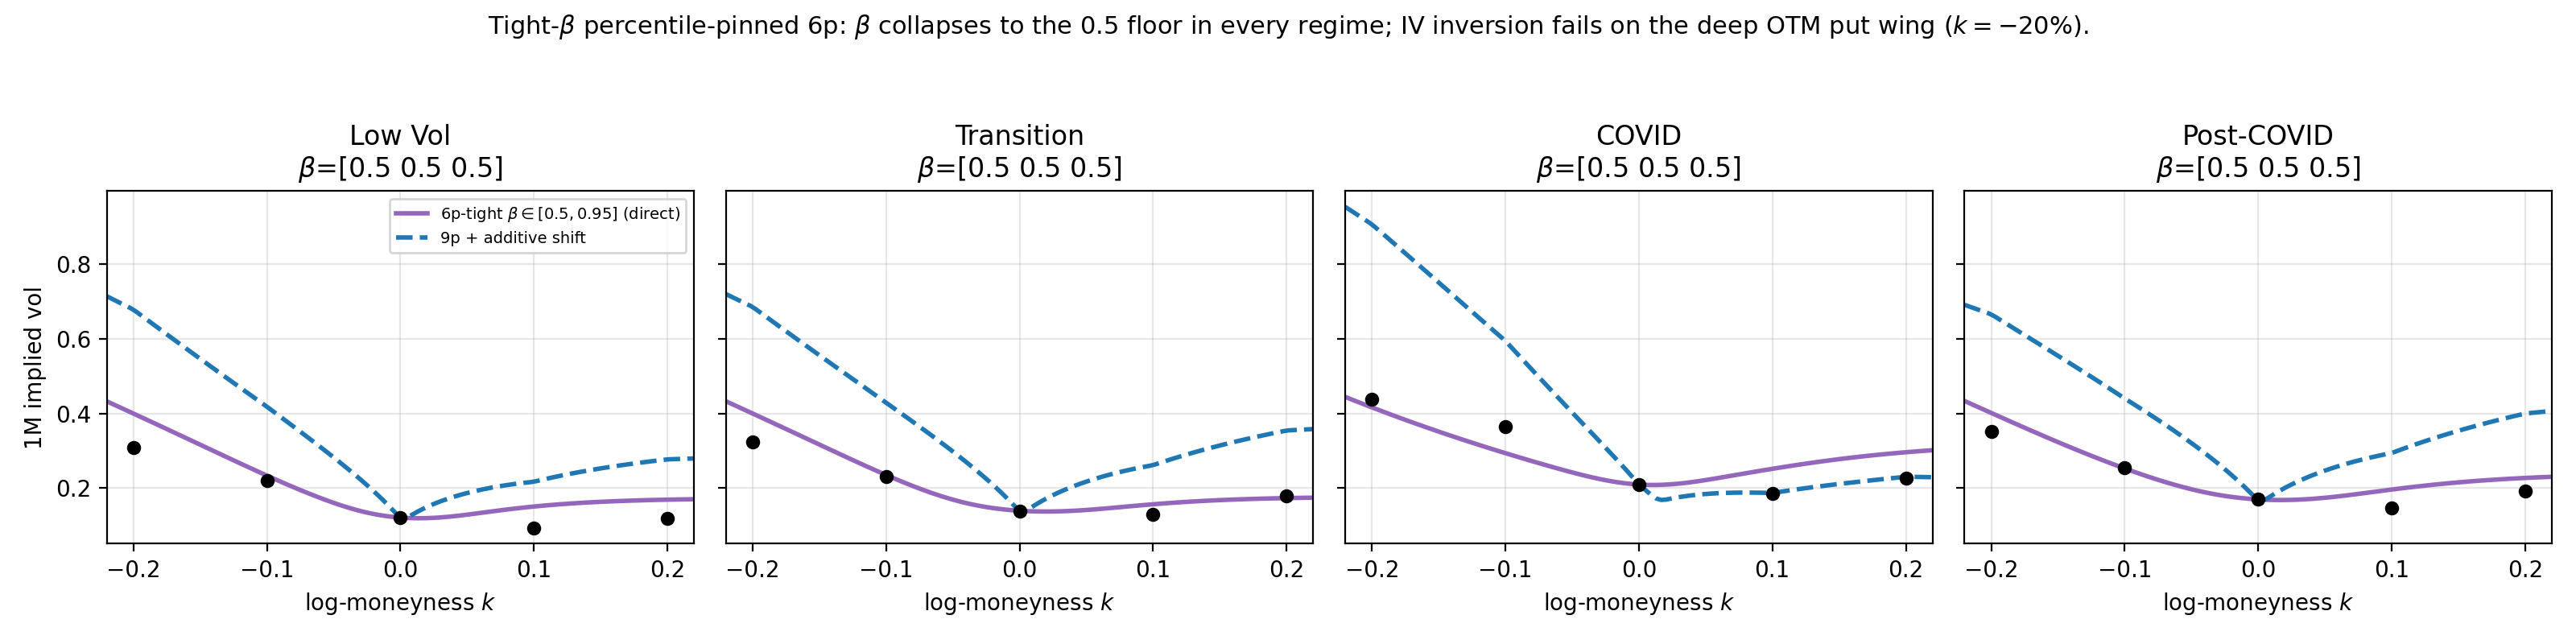
\includegraphics[width=\textwidth]{robust_percentile_6p_tight_failure.png}
  \caption{6p-tight ($\beta \in [0.50,0.95]$): $\beta$ collapses to the $0.50$ floor in every regime (sub-titles) and the IV inversion fails on the deep-OTM put wing ($k=-0.20$, shaded red). The ATM MSE is also worse than 6p/9p in every regime.}
  \label{fig:6p_tight}
\end{figure}

\paragraph{Why it was abandoned.} Fixing $\sigma$ alone cannot retire the additive shift. The degeneracy of the ATM-only loss is structural, not parametric: a single one-point-per-day ATM observation does not identify three states, regardless of whether $\sigma$ is free or pinned. The optimiser will find a corner of the remaining 6-dimensional feasible set---one-hot weights, floored $\beta$, floored-and-clipped $\beta$---and produce a smile that looks reasonable at $K=S$ but is wrong in shape everywhere else. The lesson: a smile-shaped constraint must be enforced inside the loss, not hoped for as a side-effect of pinning. This is precisely what the joint calibration of Section~\ref{sec:joint} does.

\subsection{Price-Level (Bachelier) Parameterisation}
\label{sec:robust_pricelevel}

\paragraph{Motivation.} A natural alternative to the displaced-diffusion (log-moneyness) mixture is a pure Bachelier (price-level) mixture: three states with three softmax weights and three normal volatilities $\sigma_{N,i}$---six parameters in total, no displacement. The motivation is parsimony: if the ATM backbone is well described by a single effective normal vol, the Bachelier mixture should fit equally well and be simpler to estimate. We tested this directly.

\paragraph{The ATM Bachelier call is structurally unidentifiable.} At $K=S$ the Bachelier call is
\begin{equation}
  C_{\text{Bach}}(S{=}K,\,r,\,\sigma_{N},\,T) = e^{-rT}\,\sigma_{N}\sqrt{T}\,\phi(0),
\end{equation}
and under the mixture
\begin{equation}
  C_{\text{mix}} = e^{-rT}\sqrt{T}\,\phi(0)\cdot \sum_{i=1}^{3} w_i\,\sigma_{N,i}.
\end{equation}
The mixture depends on the states only through $\sum w_i\sigma_{N,i}$, so the states are observationally equivalent to a single state with $\sigma_{\text{eff}} = \sum_i w_i \sigma_{N,i}$. The optimiser is free to push the weights to any corner of the simplex that produces the same weighted sum.

\paragraph{Empirical degeneracy.} In three of four regimes the optimiser collapses the weights to $(\approx 0, \approx 0, 1.0)$, reducing the model to a single-state Bachelier. The $\sigma_N$ remain stuck at their initial conditions $\{50,150,400\}$ in price/$\sqrt{\text{yr}}$ units because only the weighted sum matters. The MSE differences against the 9-parameter fit are within $\pm 10\%$ (Table~\ref{tab:comparison})---as they must be, since at ATM both parameterisations reduce to fitting one effective volatility.

\begin{table}[htbp]
\centering
\caption{MSE comparison: log-moneyness (9 params) vs price-level (6 params). All differences are within $\pm 10\%$, consistent with ATM-only unidentifiability of the Bachelier mixture.}
\label{tab:comparison}
\begin{tabular}{lccc}
\toprule
Regime & Log-Moneyness MSE & Price-Level MSE & $\Delta$ MSE \\
\midrule
Low Vol (2015--17) & 0.000795 & 0.000722 & $-9.2\%$ \\
Transition (2018--19) & 0.000907 & 0.000904 & $-0.3\%$ \\
COVID (2020) & 0.005632 & 0.005488 & $-2.6\%$ \\
Post-COVID (2021--25) & 0.002463 & 0.002549 & $+3.5\%$ \\
\bottomrule
\end{tabular}
\end{table}

\begin{figure}[htbp]
  \centering
  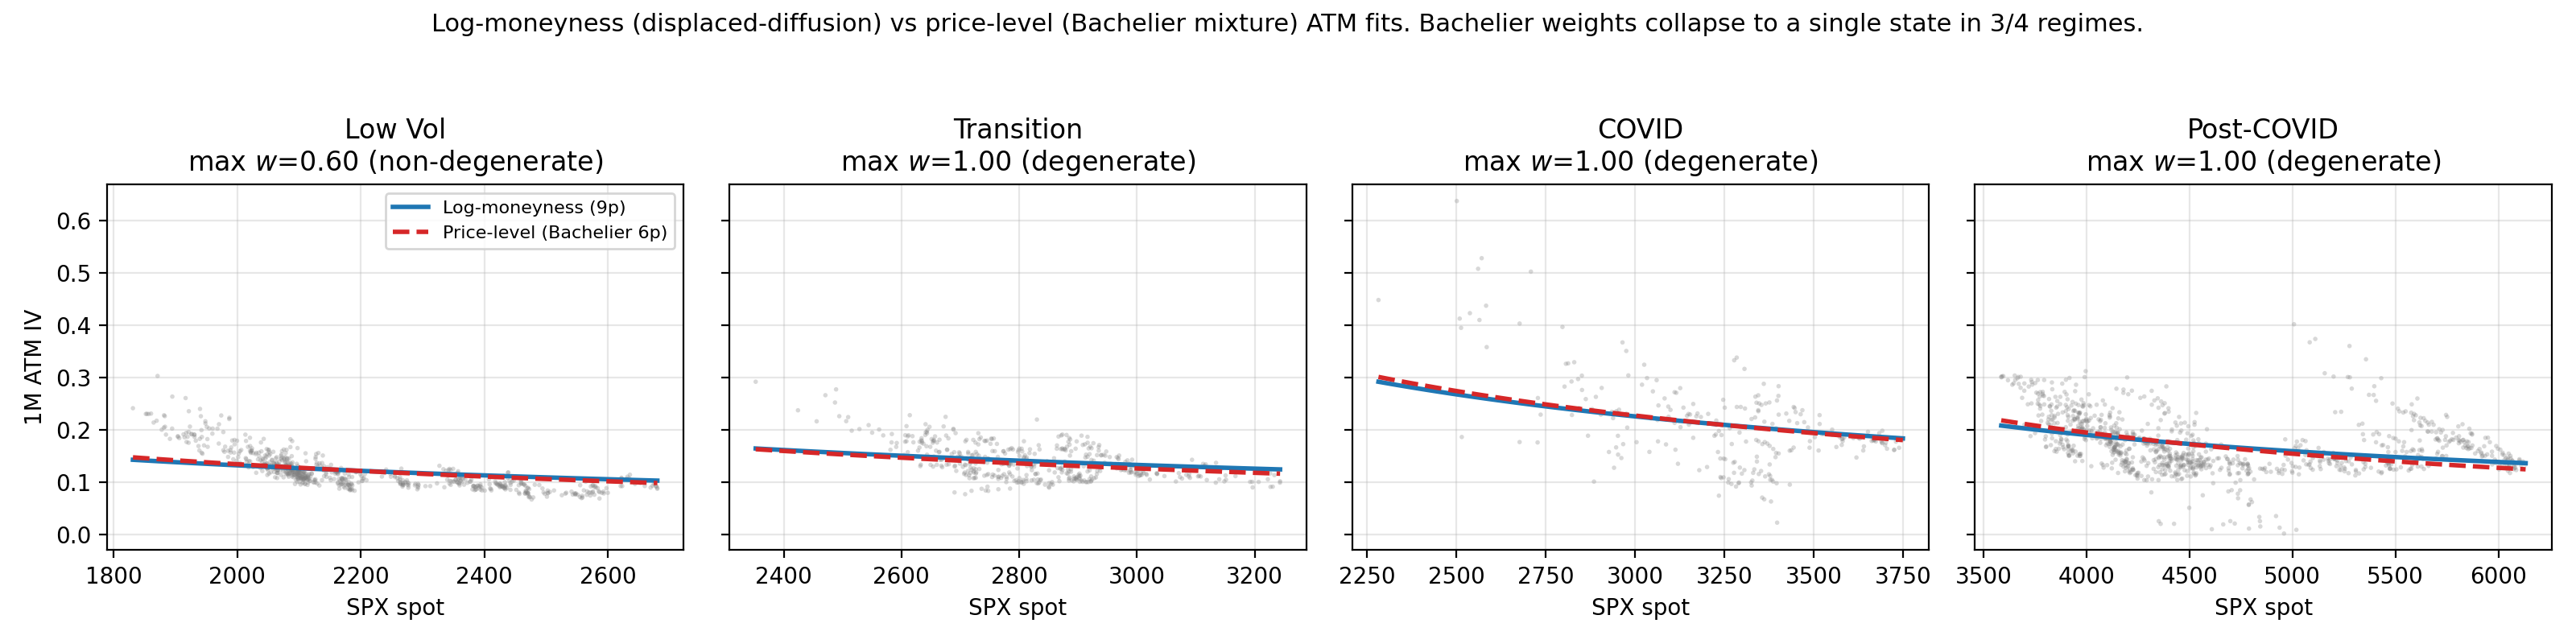
\includegraphics[width=\textwidth]{robust_price_level_degeneracy.png}
  \caption{Log-moneyness (displaced-diffusion, 9p) vs price-level (Bachelier, 6p) ATM fits. The Bachelier weights collapse to a single state ($\max w \approx 1$) in 3 of 4 regimes; the log-moneyness $\beta$ structure prevents the collapse.}
  \label{fig:pricelevel}
\end{figure}

\paragraph{Why the log-moneyness model is preferred.} The displaced-diffusion $\beta$ parameter creates distinguishable payoff profiles at $S=K$ even when $\sigma_{\ln}$ is at the floor: the displacement shifts $S$ and $K$ by state-specific amounts, so two states with different $\beta$ produce genuinely different prices. This is what prevents the log-moneyness model from collapsing to one state at ATM. Away from ATM, $\beta$ generates skew; the Bachelier mixture is flat by construction and cannot produce a smile. The six-parameter Bachelier specification is therefore \emph{not} a viable alternative: it is unidentifiable at ATM and skewless away from it. The three extra $\beta$ parameters of the displaced-diffusion model are not wasted overhead---they are what makes the joint calibration of Section~\ref{sec:joint} identifiable at all.

\begin{table}[htbp]
\centering
\caption{Decision criteria: log-moneyness (displaced-diffusion) vs price-level (Bachelier).}
\label{tab:decision}
\small
\begin{tabular}{lcc}
\toprule
Criterion & Log-Moneyness & Price-Level \\
\midrule
ATM fit quality & Same & Same \\
Parameter identifiability at ATM & Yes ($\beta$ creates separation) & No (degenerate) \\
OTM extension & Natural skew via $\beta$ & Flat (no skew) \\
Parsimony & 9 params & 6 params (3 unused) \\
\bottomrule
\end{tabular}
\end{table}


\section{Self-Critique and Open Questions}
\label{sec:critique}

Several aspects of the current analysis warrant scrutiny:

\paragraph{Asymmetric interpolation bias.} The held-out $k=\pm 0.10$ bias is systematic and asymmetric in every regime (model underprices OTM puts, overprices OTM calls). This is the most actionable limitation of the joint calibration: the three-state displaced-diffusion smile is too symmetric/linear between the trained strikes. A four-state mixture, an additional curvature degree of freedom per state, or a different functional family for the mixture components is the obvious next step; the consistency of the bias sign across regimes is a useful guide for choosing which.

\paragraph{One redundant state.} Each regime pins one $\beta$ to the upper bound in the joint fit and at least one $\sigma_{\ln}$ to the floor; in COVID the third state becomes a near-duplicate of the second. The three-state structure is therefore slightly over-parameterised for SPX; a more parsimonious two-state displaced-diffusion mixture, or a four-state mixture with an explicit intermediate-skew state, would both be natural refinements to test.

\paragraph{Dead states still die at the floor.} Although the joint fit no longer has \emph{two} dead $\sigma_{\ln}$, it still has one ($\sigma_{\ln,1}=0.01$ in COVID). The ``uncertain volatility'' interpretation is thus still partly retrospective---the model does not genuinely mix three live states at every point in time, even when OTM information is available. This is a genuine weakness of the family, not just of the calibration.

\paragraph{Year-based regime definitions.} Using year thresholds (2017, 2019, 2020) is ad hoc. PELT change-point detection on the IV series would yield data-driven boundaries, but we have not yet verified whether this materially changes the parameter estimates or the interpolation bias.

\paragraph{No term structure.} The analysis uses one-month options ($\tau = 30/365$) only. Whether the joint-calibrated smile and its interpolation bias extrapolate to other tenors is open; early evidence suggests the backbone slope and curvature change with maturity, so a 3D (spot, moneyness, tenor) surface is the natural extension.

\paragraph{$\beta_k \approx 1$ without a formal test.} The additive-shift subsection (\ref{sec:robust_additive}) rests on an informal near-unity slope of OTM IV on ATM IV; we did not compute per-moneyness $\beta_k$ and $R^2$ with a held-out procedure. The joint calibration removes this dependency---it is justified by the held-out $k=\pm 0.10$ interpolation test instead---but the gap remains in the robustness section's own justification, and we flag it as a deferred check rather than a closed one.

\paragraph{MSE vs MAE.} Our choice of MSE is deliberate (Section~\ref{sec:mse}) but not beyond question. MAE is more robust to the very outliers (COVID crash days) that MSE emphasises. A formal comparison on held-out data, including out-of-sample backtesting of the held-out interpolation bias, would strengthen this choice.

\paragraph{Stationarity within regimes.} The model treats each regime as stationary. Within-regime parameter drift---especially during COVID---is not captured. A time-varying or stochastic-weight extension could address this but would require a different estimation approach.

\paragraph{Bitcoin as future work.} The BTC extension was scoped (BTC-settled pricing formulas, a Deribit download/processing pipeline, and an SPX-mirrored analysis notebook) but is not reported here: at the time of writing, the freely available Deribit trade data has gaps at OTM strikes around the 08:00 UTC daily snapshot, and the joint calibration relies on a complete cross-section at the training moneyness levels. Tick-level order-book snapshots would resolve this, but we do not have a multi-year such record. We therefore defer the BTC backbone to future work rather than present a partial ATM-only BTC result that would repeat the very dead-state problem this paper exists to solve.


\section{Conclusions}
\label{sec:conclusion}

We have presented a joint ATM--OTM calibration with interpolation as a core methodology for the uncertain-volatility backbone, applied to one-month SPX implied volatility across four regimes from 2015 to 2025. The same nine displaced-diffusion parameters per regime, fitted simultaneously to $k \in \{-0.20, 0, +0.20\}$, reproduce the OTM smile \emph{endogenously} and retire the ad hoc additive shift required by ATM-only calibrations. The held-out strikes $k \in \{-0.10, +0.10\}$ test the mixture's interpolation, exposing a small but consistent asymmetric bias (under-priced $k=-0.10$, over-priced $k=+0.10$) that points directly to the limitation of the three-state specification: its smile is too linear between trained strikes.

The principal findings are:
\begin{enumerate}
  \item \textbf{The joint calibration retires the additive shift on the trained strikes.} The model reproduces the $k=\pm 0.20$ IV directly from $K = S e^{k}$; the additive-shift overlay, while still exact-on-mean, becomes a benchmark rather than the methodology (Figures~\ref{fig:joint_closeup}--\ref{fig:joint_pm20}).
  \item \textbf{Adding OTM data does not distort the backbone.} The ATM curve from the joint fit coincides with the ATM-only backbone (Figure~\ref{fig:joint_vs_atm}); the OTM degrees of freedom entered the smile shape, not the backbone---the joint loss is well-conditioned.
  \item \textbf{The displaced-diffusion parameterisation is essential, not ornamental.} The Bachelier (price-level) mixture is unidentifiable at ATM (weights collapse to a single state) and skewless away from ATM; the extra three $\beta$ parameters are what makes the joint calibration identifiable and what generates the smile (Section~\ref{sec:robust_pricelevel}).
  \item \textbf{Patching the dead-state problem after the fact does not work.} Additive shifts, percentile-pinned $\sigma$, and tight-$\beta$ variants each relocate the degeneracy---from $\sigma \to$ floor, to weights $\to$ one-hot, to $\beta \to$ floor---or fail numerically on the deep-OTM put wing. Only a smile-shaped constraint \emph{inside} the loss (the joint ATM--OTM MSE) addresses the cause (Section~\ref{sec:robust}).
  \item \textbf{The three-state mixture is slightly over-parameterised for SPX.} Each regime pins one $\beta$ to the upper bound and at least one $\sigma_{\ln}$ to the floor; a two- or four-state refinement is the natural next specification.
\end{enumerate}

Future work should address (i) the asymmetric interpolation bias via a richer mixture or alternative component family, (ii) data-driven (PELT) regime detection, (iii) a term-structure extension to a 3D smile surface, (iv) formal out-of-sample backtesting of the held-out interpolation, and (v) the Bitcoin backbone estimation once sufficient cross-sectional OTM data is available.


\clearpage

\singlespacing \bibliography{refs}



\end{document}